\documentclass[a4paper, twoside, 11pt]{article}
% It is needed to use this command for automatic compilation in VSCode
% !TEX program = lualatexmk

%% DOCUMENT, PREAMBLE AND MACROS DESIGNED FOR LuaLaTeX %%
\newcommand{\fbar}{\FloatBarrier} % barier for stopping figures from leaking to other subsections, use as \fbar


\usepackage{amsmath} % math package
\usepackage{amssymb} % for miscellaneous mathematical symbols, first usage was for tick symbol in math mode \checkmark
\usepackage{textcomp} % for miscellaneous symbols
\usepackage{graphicx} % enhanced support for graphics
\usepackage{cmap} % mapování znaků - vyhledávání v pdf
% \usepackage[czech]{babel} % CZ
\usepackage[english]{babel} % EN
\usepackage[utf8]{inputenc} % kódování 
\usepackage[T1]{fontenc} % kódování 
\usepackage{multirow} % Multirow table support
\usepackage{float} % Improves the interface for defining floating objects such as figures and tables
\usepackage{wasysym} % for various glyphs, symbols
\usepackage{subcaption}
\usepackage{setspace} % spacing
\onehalfspacing

\usepackage{hyperref}
\hypersetup{
    colorlinks=true, % pokud nechci definovat citecolor=black aby byly odkazy citací černé, tak dám colorlinks=false,%
    bookmarks=true,
    linkcolor=black,
    citecolor=black,
    urlcolor=black,
    pdfauthor={Petr Zakopal},
    pdftitle={A Brief Report on Permanent Magnet Assisted Synchronous Reluctance Motors},
    pdfsubject={XP14DES},
    pdfkeywords={},
    pdfproducer={},
    pdfcreator={}
}

% when using LuaLaTex, defining Times Fonts from your system - it has to be named like this and inserted ttf file in the folder of your tex file
\usepackage{fontspec}
\selectlanguage{czech}
\setmainfont[Ligatures=TeX,BoldFont={Times New Roman Bold}] {Times New Roman}
                                
\setsansfont[Ligatures=TeX,BoldFont={* Bold}]{Times New Roman}
                                      
\setmonofont{CourierPrime-Regular}
 
%\usepackage[italic]{mathastext} % for text in math environment, better looking times then



% for CITATIONS URL to work, it is not needed when you are not using URL label
\usepackage{url}
\usepackage{csquotes}
\usepackage[style=iso-numeric, backend=biber, isbn=true, urldate=iso,seconds=true, date=terse, datezeros=true, language=czech]{biblatex}
\addbibresource{src/bib/zdroje.bib} % BIB resources to import
%\DeclareUrlCommand\url{\def\UrlLeft{<}\def\UrlRight{>} \urlstyle{tt}}
%\usepackage{biblatex}
% END for citations %

% changing bibliography font
\renewcommand*{\bibfont}{\fontspec{Times New Roman}}

\usepackage{comment} % For comments
\usepackage{pdfpages} % for pdf pages
\usepackage{enumerate} % For lists
\usepackage{enumitem} % For Custom Numbering Nested Lists
\setlist[enumerate]{label*=\arabic*.} % setting Number. numbering in lists
\usepackage{tikz} % For vector graphics
\usepackage{circuitikz} % For schemes
\usepackage{pgf} % Post script graphics for tikz

% pouze funguje v PDFLaTeX%
%\usepackage{tgtermes} % na times font, jiný nefunguje s vyhledáváním a copy%

\usepackage{placeins} % for \FloatBarrier command that blocks floating with htbp! go over \FloatBarrier
\usepackage{mathrsfs} % package for math symbols for Laplace, Z transform etc., usage \mathscr{Z}
\usepackage{upgreek} % for upgreek symbols, specified tau \uptau
\usepackage{physics} % for derivations \dd
\usepackage[list=true,listformat=simple]{subcaption}
\usepackage[figurename=Fig.,font=small,labelfont=it,textfont=it]{caption} %for renaming figures instead of renewcommand, small for 11pt default is 10pt as needed in word template
\usepackage[tablename=Tab.,font=small,labelfont=it,
            textfont=it]{caption} % for renaming tables instead of renewcommand
            

%% GLOSSARIES %%
% List of abbreviations and symbols
% Original code author: Jakub Kučera

\usepackage[nonumberlist,nopostdot,section=subsection,numberedsection]{glossaries}
% section = subsection is for glossaries title to appear as a subsection, numberedsection adds the subsec number

\newglossary[slg]{symbolslist}{symbol}{ntn1}{List of symbols}
\newglossary[slg]{abbreviationslist}{abbreviation}{ntn2}{List of abbreviations}

\makeglossaries

% include files with definitions
% PZ definitions
\newglossaryentry{abbreviation:asm}{
                type=abbreviationslist,
                name={ASM},
                description={Asynchronní Motor}
}
\newglossaryentry{abbreviation:pmsynrelm}{
                type=abbreviationslist,
                name={PMSynRelM},
                description={Permanent Magnet Assisted Synchronous Reluctance Motor}
}
\newglossaryentry{abbreviation:synrelm}{
                type=abbreviationslist,
                name={SynRelM},
                description={Synchronous Reluctance Motor}
}
\newglossaryentry{abbreviation:pm}{
                type=abbreviationslist,
                name={PM},
                description={Permanent Magnets}
}
\newglossaryentry{abbreviation:pmsm}{
                type=abbreviationslist,
                name={PMSM},
                description={Permanent Magnet Synchronous Motor}
}
\newglossaryentry{abbreviation:dsp}{
                type=abbreviationslist,
                name={DSP},
                description={Digial Signal Processor}
}
\newglossaryentry{abbreviation:foc}{
                type=abbreviationslist,
                name={FOC},
                description={Field Oriented Control}
}
\newglossaryentry{abbreviation:dtc}{
                type=abbreviationslist,
                name={DTC},
                description={Direct Torque Control}
}
\newglossaryentry{abbreviation:mtpa}{
                type=abbreviationslist,
                name={MTPA},
                description={Maximum Torque Per Ampere}
}
\newglossaryentry{abbreviation:mtpv}{
                type=abbreviationslist,
                name={MTPV},
                description={Maximum Torque Per Voltage}
}
\newglossaryentry{abbreviation:emf}{
                type=abbreviationslist,
                name={EMF},
                description={Electromotive Force}
}
\newglossaryentry{abbreviation:upfc}{
                type=abbreviationslist,
                name={UPFC},
                description={Unity Power Factor Control}
}

\newglossaryentry{abbreviation:pwm}{
                type=abbreviationslist,
                name={PWM},
                description={Pulse Width Modulation}
}


\newglossaryentry{symbol:Pn}{
    type=symbolslist, % glossary
    name=$P_\text{n}$, % jméno v seznamu
    description={jmenovitý výkon}, %popis
    symbol = (W),
    sort=P % seředit podle
}

\newglossaryentry{symbol:Un}{
    type=symbolslist, % glossary
    name=$U_\text{n}$, % jméno v seznamu
    description={jmenovité sdružené napětí}, %popis
    symbol = (V),
    sort=U % seředit podle
}

\newglossaryentry{symbol:fn}{
    type=symbolslist, % glossary
    name=$f_\text{n}$, % jméno v seznamu
    description={jmenovitá napájecí frekvence}, %popis
    symbol = (Hz),
    sort=F% seředit podle
}

\newglossaryentry{symbol:cosphin}{
    type=symbolslist, % glossary
    name=$\cos(\varphi_\text{n})$, % jméno v seznamu
    description={jmenovitý účinník}, %popis
    symbol = (-),
    sort=P% seředit podle
}

\newglossaryentry{symbol:nn}{
    type=symbolslist, % glossary
    name=$n_\text{n}$, % jméno v seznamu
    description={jmenovité otáčky}, %popis
    symbol = (min$^{-1}$),
    sort=P% seředit podle
}


\newglossaryentry{symbol:In}{
    type=symbolslist, % glossary
    name=$I_\text{n}$, % jméno v seznamu
    description={jmenovitý fázový proud stroje}, %popis
    symbol = (A),
    sort=I % seředit podle
}

\newglossaryentry{symbol:u1}{
    type=symbolslist, % glossary
    name=$\underline{u_{1}^{k}}$, % jméno v seznamu
    description={prostorový vektor napětí statorového vinutí}, %popis
    symbol = (V),
    sort=U % seředit podle
}

\newglossaryentry{symbol:u2}{
    type=symbolslist, % glossary
    name=$\underline{u_{2}^{k}}$, % jméno v seznamu
    description={prostorový vektor napětí rotorového vinutí}, %popis
    symbol = (V),
    sort=U % seředit podle
}

\newglossaryentry{symbol:psi1}{
    type=symbolslist, % glossary
    name=$\underline{\psi_1^{k}}$, % jméno v seznamu
    description={prostorový vektor spřaženého magnetického toku statorového vinutí}, %popis
    symbol = (Wb),
    sort=P % seředit podle
}

\newglossaryentry{symbol:psi2}{
    type=symbolslist, % glossary
    name=$\underline{\psi_2^{k}}$, % jméno v seznamu
    description={prostorový vektor spřaženého magnetického toku rotorového vinutí}, %popis
    symbol = (Wb),
    sort=P % seředit podle
}

\newglossaryentry{symbol:r1}{
    type=symbolslist, % glossary
    name=$R_1$, % jméno v seznamu
    description={rezistivita statorového vinutí}, %popis
    symbol = ($\Omega$),
    sort=R % seředit podle
}

\newglossaryentry{symbol:r2}{
    type=symbolslist, % glossary
    name=$R_2$, % jméno v seznamu
    description={rezistivita rotorového vinutí}, %popis
    symbol = ($\Omega$),
    sort=R % seředit podle
}

\newglossaryentry{symbol:i1}{
    type=symbolslist, % glossary
    name=$\underline{i_1^{k}}$, % jméno v seznamu
    description={prostorový vektor proudu statorového vinutí}, %popis
    symbol = (A),
    sort=I % seředit podle
}

\newglossaryentry{symbol:i2}{
    type=symbolslist, % glossary
    name=$\underline{i_2^{k}}$, % jméno v seznamu
    description={prostorový vektor proudu rotorového vinutí}, %popis
    symbol = (A),
    sort=I % seředit podle
}

\newglossaryentry{symbol:omega}{
    type=symbolslist, % glossary
    name=$\omega$, % jméno v seznamu
    description={elektrická úhlová rychlost rotoru}, %popis
    symbol = (s$^{-1}$),
    sort=O % seředit podle
}

\newglossaryentry{symbol:omegas}{
    type=symbolslist, % glossary
    name=$\omega_\text{s}$, % jméno v seznamu
    description={skluzová elektrická úhlová rychlost}, %popis
    symbol = (s$^{-1}$),
    sort=O % seředit podle
}

\newglossaryentry{symbol:omegak}{
    type=symbolslist, % glossary
    name=$\omega_\text{k}$, % jméno v seznamu
    description={obecná elektrická úhlová rychlost}, %popis
    symbol = (s$^{-1}$),
    sort=O % seředit podle
}

\newglossaryentry{symbol:omegamech}{
    type=symbolslist, % glossary
    name=$\Omega$, % jméno v seznamu
    description={mechanická úhlová rychlost}, %popis
    symbol = (s$^{-1}$),
    sort=O % seředit podle
}

\newglossaryentry{symbol:omega1}{
    type=symbolslist, % glossary
    name=$\omega_1$, % jméno v seznamu
    description={elektrická úhlová rychlost točivého magnetického pole}, %popis
    symbol = (s$^{-1}$),
    sort=O % seředit podle
}

\newglossaryentry{symbol:l1}{
    type=symbolslist, % glossary
    name=$L_1$, % jméno v seznamu
    description={indukčnost statorového vinutí}, %popis
    symbol = (H),
    sort=L % seředit podle
}

\newglossaryentry{symbol:j}{
    type=symbolslist, % glossary
    name=$J$, % jméno v seznamu
    description={moment setrvačnosti}, %popis
    symbol = (kg$\cdot$m$^{2}$),
    sort=J % seředit podle
}

\newglossaryentry{symbol:l1sigma}{
    type=symbolslist, % glossary
    name=$L_{1\sigma}$, % jméno v seznamu
    description={rozyptylová indukčnost statorového vinutí}, %popis
    symbol = (H),
    sort=L % seředit podle
}

\newglossaryentry{symbol:l2sigma}{
    type=symbolslist, % glossary
    name=$L_{2\sigma}$, % jméno v seznamu
    description={rozyptylová indukčnost rotorového vinutí}, %popis
    symbol = (H),
    sort=L % seředit podle
}

\newglossaryentry{symbol:lm}{
    type=symbolslist, % glossary
    name=$L_\text{m}$, % jméno v seznamu
    description={magnetizační indukčnost}, %popis
    symbol = (H),
    sort=L % seředit podle
}

\newglossaryentry{symbol:l2}{
    type=symbolslist, % glossary
    name=$L_2$, % jméno v seznamu
    description={indukčnost rotorového vinutí}, %popis
    symbol = (H),
    sort=L % seředit podle
}

\newglossaryentry{symbol:pp}{
    type=symbolslist, % glossary
    name=$p_\text{p}$, % jméno v seznamu
    description={počet polpárů stroje}, %popis
    symbol = (-),
    sort=P % seředit podle
}

\newglossaryentry{symbol:m}{
    type=symbolslist, % glossary
    name=$M$, % jméno v seznamu
    description={vnitřní elektromechanický moment stroje}, %popis
    symbol = (Nm),
    sort=P % seředit podle
}

\newglossaryentry{symbol:mz}{
    type=symbolslist, % glossary
    name=$M$, % jméno v seznamu
    description={zátěžný moment}, %popis
    symbol = (Nm),
    sort=P % seředit podle
}

\newglossaryentry{symbol:slip}{
    type=symbolslist, % glossary
    name=$s$, % jméno v seznamu
    description={skluz}, %popis
    symbol = (-),
    sort=S % seředit podle
}

\newglossaryentry{symbol:u1ef}{
    type=symbolslist, % glossary
    name=$U_1$, % jméno v seznamu
    description={efektivní hodnota fázového napájecího napětí}, %popis
    symbol = (V),
    sort=U % seředit podle
}


\newglossarystyle{myStyleAbbreviations}{
\renewenvironment{theglossary}%
     {\begin{longtable}[l]{llp{\glsdescwidth}p{\glspagelistwidth}}}%
     {\end{longtable}}%
  \renewcommand*{\glossaryheader}{}%
  \renewcommand*{\glsgroupheading}[1]{}%
  \renewcommand{\glossentry}[2]{%
  \glsentryitem{##1} \glstarget{##1}{##2} &
    \textbf{\glossentryname{##1}} &
    \glossentrydesc{##1} &
    ##2\tabularnewline
  }%
  \renewcommand*{\glsgroupskip}{}%  Pokud chci seskupovat podle abeced: \renewcommand*{\glsgroupskip}{ & \\}
}


\newglossarystyle{myStyleSymbols}{
  \renewenvironment{theglossary}%
    {\begin{longtable}[l]{llp{\glsdescwidth}p{\glspagelistwidth}}}%
    {\end{longtable}}%
  \renewcommand*{\glossaryheader}{}%
  \renewcommand*{\glsgroupheading}[1]{}%
  \renewcommand{\glossentry}[2]{%
    \glsentryitem{##1} \glstarget{##1}{\glossentryname{##1}} &
    \glossentrysymbol{##1} &
    \glossentrydesc{##1} &
    ##2\tabularnewline
  }%
  \renewcommand{\subglossentry}[3]{%
     &
     \glssubentryitem{##2}%
     \glossentrysymbol{##2} &
     \glstarget{##2}{\strut}\glossentrydesc{##2} & ##3\tabularnewline
  }%
  \renewcommand*{\glsgroupskip}{%
   }% Pokud chci seskupovat podel abecedy  \ifglsnogroupskip\else & & &\tabularnewline\fi
}
\renewcommand{\glossarypreamble}{\vspace*{-\baselineskip}} % deleting line after glossaries title


%% END OF GLOSSARIES %%

% this works with LuaLaTex and fontspec package %
\DeclareCaptionFont{times}{\fontspec{Times New Roman Italic}}

% labelfont and textfont defined here only works with previous declarecaptionfont times and fontspec
\captionsetup{labelfont=times, textfont=times, labelsep=space}%no separator in captions


%\bibliographystyle{czechiso} %czechiso.bst in folder is needed for this style to work, available at http://www.fit.vutbr.cz/~martinek/latex/czechiso.html%


\usepackage{chngcntr} % for numbered figures with sections
\usepackage{tocloft} % better TOC

%\usepackage{a4wide}%širší a4%
\usepackage[inner=3cm,outer=2cm,top=2.5cm,bottom=2.5cm,footskip=1cm]{geometry}%for propper margins
\usepackage{textcase} % for making text uppercase without caps \MakeTextUppercase
 
 
\usepackage{titlesec} % for spacing text after sections
\usepackage{parskip}[] % for working \parskip
%\newcommand{\sectionbreak}{\clearpage} % maybe for SECTIONS on a new page

\usepackage[titletoc]{appendix} % For appendix - přílohy, titletoc is crucial
%\renewcommand{\appendixname}{Příloha}

\setlength{\parindent}{0.5cm} % setting indent of paragraph to 0.5cm
\setlength{\parskip}{0em} % setting parskip to 0 for \titleformat to work properly with parskip package

\usepackage{colortbl} % for colored cells in tables
\usepackage{xcolor} % for color definitions

%% COLOR DEFINITIONS %%
\definecolor{ctublue}{HTML}{0065BD} % defining ctu color
\definecolor{ctugreen}{HTML}{A2AD00}
\definecolor{ctured}{HTML}{C60C30}
\definecolor{ctuyellow}{HTML}{F0AB00}
\definecolor{ctugreenyblue}{HTML}{00B2A9}
\definecolor{ctulightblue}{HTML}{6AADE4}
\definecolor{ctuorange}{HTML}{E05206}
\definecolor{lightgray}{HTML}{D1D5DB}
\definecolor{codeblue}{HTML}{D9E2F3}
\definecolor{codegreen}{rgb}{0,0.6,0}
\definecolor{codegray}{rgb}{0.5,0.5,0.5}
\definecolor{codepurple}{rgb}{0.58,0,0.82}
\definecolor{backcolour}{rgb}{0.95,0.95,0.92}

% defining spacing of titles
\titlespacing*{\section}{0em}{1em}{-\parskip} % spacing text after sections from titlesec package
\titlespacing*{\subsection}{0em}{1em}{-\parskip} % spacing text after sections from titlesec package
\titlespacing*{\subsubsection}{0em}{1em}{-\parskip} % spacing text after sections from titlesec package

% defining style for titles
% when you want section/sub/subsub to be black, delete \color{ctublue}
\titleformat{\section}{\color{ctublue}\fontspec{Times New Roman}\fontsize{15}{15}\bfseries}{\thesection}{2.1em}{}%defining title sizes by word template
\titleformat{\subsection}{\color{ctublue}\fontspec{Times New Roman}\fontsize{14}{14}\bfseries}{\thesubsection}{1.53em}{}%defining title sizes by word template
\titleformat{\subsubsection}{\color{ctublue}\fontspec{Times New Roman}\fontsize{13}{13}\bfseries}{\thesubsubsection}{1em}{}%defining title sizes by word template


\usepackage{ctable} % imports xtable with booktabs
\usepackage{multicol} % for multicolumn feature in tables

\usepackage{listings} % for code environments - \begin{lstlisting}

% solving problems with ) literal to be coded in lstlisting as it should be
\makeatletter
\patchcmd{\lsthk@SelectCharTable}{)}{`}{}{} 
\makeatother 

\lstdefinestyle{zakopal}{
    backgroundcolor=\color{codeblue},   
    commentstyle=\color{codegray},
    keywordstyle=\color{ctured},
    numberstyle=\tiny\color{codegray},
    stringstyle=\color{ctuorange},
    basicstyle=\ttfamily\small,
    breakatwhitespace=false,         
    breaklines=true,                 
    captionpos=b,                    
    keepspaces=true,                 
    numbers=left,                    
    numbersep=5pt,                  
    showspaces=false,                
    showstringspaces=false,
    showtabs=false,                  
    tabsize=2
}
\lstset{style=zakopal}
\renewcommand{\lstlistingname}{Code}% renaming Listing -> Kód 
\renewcommand{\lstlistlistingname}{List of codes}% renaming List of Listings -> Seznam kódů

\lstdefinelanguage{SCL}
{morekeywords={FUNCTION_BLOCK,BEGIN,NOT,END_FUNCTION_BLOCK,FUNCTION,VOID,VAR_INPUT,END_VAR,VAR_IN_OUT,IF,
THEN,END_IF,END_FUNCTION,BOOL,FALSE,TRUE},
sensitive=false,
morecomment=[l]{//},
morestring=[b]",
literate={;}{{\textcolor{ctuorange}{;}}}{1}
{:}{{\textcolor{ctuorange}{:}}}{1}
{)}{{\textcolor{ctuorange}{)}}}{1}
{(}{{\textcolor{ctuorange}{(}}}{1}
{=}{{\textcolor{ctuorange}{=}}}{1}
{,}{{\textcolor{ctuorange}{,}}}{1},} %basic SCL language for siemens defined%

\lstdefinelanguage{xdc}
{morekeywords={set_property, current_design, get_ports},
sensitive=false,
morecomment=[l]{\#}} %basic xdc file in Vivado syntax highlighting%

\lstdefinelanguage{xsct}
{morekeywords={xsct, hsi, open_hw_design, -createdts, -hw, -zocl, -platform-name, -overlay, -compile, -out, exit, -git-branch},
alsoletter={-},
sensitive=false,
morecomment=[l]{\#}} %xsct (Xilinx Software Command-Line Tools)%


\lstdefinelanguage{Text}
{morekeywords={},
alsoletter={-},
sensitive=false,
morecomment=[l]{//},
morecomment=[l]{\#}} %basic text%

\lstdefinelanguage{devicetree}
{morekeywords={chosen, bootargs, stdout-path, compatible, status},
alsoletter={-},
stringstyle=\color{ctuorange},
moredelim=[s][\color{ctuorange}]{"}{"},
sensitive=false,
morecomment=[l]{\#},
literate={\{}{{\textcolor{ctured}{\{}}}{1}
{\}}{{\textcolor{ctured}{\}}}}{1}
} %devicetree%

\lstdefinelanguage{json}
{morekeywords={},
upquote=true,
morestring=[b]",
stringstyle=\color{ctuorange},
moredelim=[s][\color{ctuorange}]{"}{"},
sensitive=false,
morecomment=[l]{\#},
literate=
     *{0}{{{\color{ctured}0}}}{1}
      {1}{{{\color{ctured}1}}}{1}
      {2}{{{\color{ctured}2}}}{1}
      {3}{{{\color{ctured}3}}}{1}
      {4}{{{\color{ctured}4}}}{1}
      {5}{{{\color{ctured}5}}}{1}
      {6}{{{\color{ctured}6}}}{1}
      {7}{{{\color{ctured}7}}}{1}
      {8}{{{\color{ctured}8}}}{1}
      {9}{{{\color{ctured}9}}}{1}
      {\{}{{{\color{ctured}{\{}}}}{1}
      {\}}{{{\color{ctured}{\}}}}}{1}
      {[}{{{\color{ctured}{[}}}}{1}
      {]}{{{\color{ctured}{]}}}}{1},
} %json%

\lstdefinelanguage{pseudocode}
{morekeywords={if, else, positive, negative, edge, end},
alsoletter={-},
stringstyle=\color{ctuorange},
moredelim=[s][\color{ctuorange}]{"}{"},
sensitive=false,
morecomment=[l]{\//},
literate={\{}{{\textcolor{ctured}{\{}}}{1}
{\}}{{\textcolor{ctured}{\}}}}{1}
{(}{{{\color{ctured}{(}}}}{1}
{)}{{{\color{ctured}{)}}}}{1}
} %devicetree%


%%change in previous commands 2.1 em , 1.53em and 1em to 1em to be easy indented not the same
\begin{document}
\fontspec{Times New Roman}

\counterwithin{figure}{section}%changing counter of figure, at each section the numbering resets
\counterwithin{table}{section}%changing counter of table, at each section the numbering resets
\counterwithin{equation}{section}%changing counter of equation, at each section the numbering resets

\counterwithin{lstlisting}{section}%counter of lstlist - codes, reseting at each section%


\renewcommand{\thefigure}{\thesection~-~\arabic{figure}}%defining style of countering
\renewcommand{\thetable}{\thesection~-~\arabic{table}}
\renewcommand{\theequation}{\thesection~-~\arabic{equation}}
\renewcommand{\thelstlisting}{\thesection~-~\arabic{lstlisting}}%delfining style for lstlisting codes, needs to be after begin document as previous renewcommand%

\renewcommand*{\cftsecdotsep}{1}  % use dots in the section entries and their step
\renewcommand*{\cftsubsecdotsep}{1}
\renewcommand*{\cftsubsubsecdotsep}{1}
\renewcommand*{\cftsecnumwidth}{4em} % increase space for Roman numerals
\renewcommand*{\cftsubsecnumwidth}{4em} %numbering width
\renewcommand*{\cftsubsubsecnumwidth}{4em} %numbering width
\renewcommand*{\cftsubsubsecindent}{0em}%no indent for subsubsection
\renewcommand*{\cftsubsecindent}{0em}%no indent for subsection
\renewcommand*{\cftsecindent}{0em}%no indent for subsection



\renewcommand*{\cftfigdotsep}{1}  % use dots in the figure entries and their step
\renewcommand*{\cftfignumwidth}{4em}
\renewcommand*{\cftfigindent}{0em}

\renewcommand*{\cfttabdotsep}{1}  % use dots in the figure entries and their step
\renewcommand*{\cfttabnumwidth}{4em}
\renewcommand*{\cfttabindent}{0em}

\renewcommand{\cftsecfont}{\fontspec{Times New Roman}\large \bfseries}
\renewcommand{\cftsubsecfont}{\fontspec{Times New Roman}}
\renewcommand{\cftsubsubsecfont}{\fontspec{Times New Roman}}

\renewcommand{\cftfigfont}{\fontspec{Times New Roman}}
\renewcommand{\cfttabfont}{\fontspec{Times New Roman}}

\renewcommand*\contentsname{\textcolor{ctublue}{\MakeTextUppercase{\fontspec{Times New Roman}Table of Contents}}}
\renewcommand{\listtablename}{{\fontspec{Times New Roman}\textcolor{ctublue}{\MakeTextUppercase{{List of tables}}}}}
\renewcommand{\listfigurename}{{\fontspec{Times New Roman}\textcolor{ctublue}{\MakeTextUppercase{{List of figures}}}}}


%% TITLE PAGE %%
\setcounter{figure}{0}

\begin{titlepage}
	\begin{center}

\begin{figure}[H]
	\begin{center}
		
\includegraphics[scale=1]{src/misc/symbol_cvut_konturova_verze.pdf}
	\end{center}
\end{figure}
	{\Large{\textbf{CZECH TECHNICAL UNIVERSITY IN PRAGUE}}}\\
	{\textbf{Faculty of Electrical Engineering}}\\
	{\textbf{Department of Electric Drives and Traction}}
	
	\vspace{3cm}
	
	
	{\Large\textbf{Title}}
	
	\vspace{1cm}
	
	%{\Large\textbf{Possibilities of Using SoC Platform Processors for Controlling Electric Drives}}
	
	%\vspace{2cm}
	
	Subtitle\\
	
	\end{center}
	
	\vspace{3cm}
	
	%\noindent Studijní program: Elektrotechnika, Energetika a Management\\
	%\noindent Studijní obor: Elektrické pohony
	
	\vspace{0.5cm}
	%\noindent Vedoucí práce: doc. Ing. Jan Bauer, Ph.D.
	
	\vfill
	
\begin{center}

	\large{\textbf{Petr Zakopal}}\\
	\large{\textbf{Prague 2023}}
	\end{center}
\end{titlepage}


\newpage
\pagenumbering{gobble} %disabling page numbering

\newpage


%%ZADÁNÍ PRÁCE
%verze pro TISK - jen s NEW PAGE


%ONLINE VERZE - se zadáním BEZ PODPISŮ
% online verze - odkomentovat následující dva řádky
%\null\newpage
%\includepdf[]{src/docs/zadani_bez_podpisu.pdf}

%\newpage
%\cleardoublepage
\null\newpage

\pagenumbering{Roman}
\setcounter{page}{2}%%3 NUTNO řešit dle zadání etc.

%% PROHLASENI A PODEKOVANI %%
%  \noindent \textcolor{ctublue}{{\Large{\textbf{\MakeTextUppercase{Prohlášení}}}}}\\
 			Prohlašuji, že jsem předloženou práci vypracoval samostatně a že jsem uvedl veškeré použité informační zdroje v~souladu s~Metodickým pokynem o~dodržování etických principů při přípravě vysokoškolských závěrečných prací.\\
 		\vspace{1.5cm}
		
	

 	\noindent	V~Praze dne \rule{3.5cm}{0.4pt} \hspace{6.6cm}  \rule{4cm}{0.4pt}
	
 	\hspace{12.65cm}Petr Zakopal


 		\vspace{14cm}
		
 	\noindent	\textcolor{ctublue}{{\Large{\textbf{\MakeTextUppercase{Poděkování}}}}}\\
 	Tímto bych rád poděkoval vedoucímu této práce doc. Ing. Janu Bauerovi, Ph.D. za skvělé vedení práce a cenné rady při jejím vytváření. Dále bych rád poděkoval všem, kteří mě v~mém dosavadním studiu podporovali.
	


%%ABSTRAKT%%
%  \newpage
 %\addcontentsline{toc}{section}{3\quad Abstrakt a klíčová slova}%Added citations to TOC%
 %\begin{comment}
 \begin{minipage}[t]{7.37cm}
 		\raggedright
 	\textcolor{ctublue}{\Large{\textbf{\MakeTextUppercase{Abstrakt}}}}\\
    Textík.
	
 \end{minipage}%
 \hfill% --- important, otherwise it wont be so nice
 \begin{minipage}[t]{7.37cm}
 		\textcolor{ctublue}{\Large{\textbf{\MakeTextUppercase{Abstract}}}}\\
	Textík v aj.	
 \end{minipage}
% %\end{comment}
% 	%\textcolor{ctublue}{\Large{\textbf{\MakeTextUppercase{Abstrakt}}}}\\

% 	%\textcolor{ctublue}{\Large{\textbf{\MakeTextUppercase{Abstract}}}}\\

% \newpage



%% TABLE OF CONTENTS %%
\tableofcontents
\newpage%
\flushbottom % vyčištění stránky
\newpage
\vspace{0pt}

%% LIST OF FIGURES %%
\listoffigures % seznam obrázků
\flushbottom % vyčištění stránky
\newpage

%% LIST OF TABLES %%
%\listoftables
%\flushbottom

%\newpage


%% BLANK PAGE AFTER TOC, TOF, TOT %%
\pagenumbering{gobble}
\null\newpage

% setting the page numbering to start from 1, where the main text starts
\setcounter{page}{1}
\pagenumbering{arabic}

\section{Introduction}
This concise report provides a comprehensive overview of Permanent Magnet Assisted Reluctance Motors (\gls{abbreviation:pmsynrelm}),  focusing on essential information to maintain clarity and conciseness. While the covered parts could be expanded further, the brevity of the paper is intentionally preserved to ensure its readability and clarity.\par
Nowdays the \gls{abbreviation:pmsynrelm} is being actively used in the automotive and traction applications and for its simplicity, performance and emerging availability could be used in modern electric vehicles. \par
The references used in this paper were selected based on the criteria such as rating, relevance and publication date. This approach ensures that the paper reflects modern trends in the field to the fullest extent. But certain principles used when designing or controlling \gls{abbreviation:pmsynrelm} drive were developed in earlier publications when the \gls{abbreviation:pmsynrelm} structure was not popular as nowdays is. But the controlling principles developed still work and are being improved for todays application requirements.\par
This paper is organized as follows: Firstly the most used design of the stator and rotor with permanent magnets is presented. Then the general mathematical model used for controlling the machine with corresponding strategies for \gls{abbreviation:pmsynrelm} and other permanent magnet machines are briefly explained. The next section is dedicated to comparing the \gls{abbreviation:pmsynrelm} to other popular motor structures used in the automotive and traction field. The paper ends with section briefly presenting the latest research interests in the field of \gls{abbreviation:pmsynrelm} drives.

\newpage
\section{Design}
The (\gls{abbreviation:pmsynrelm}) is widely used for its significant advantages of small size, low losses, high efficiency, wide constant power range and better performance than general synchronous reluctance motors \gls{abbreviation:synrelm}. \cite{xinmin-design-of-permanent-magnet-assisted-synch-rel-m-with-low-torque-ripple,huynh-design-and-analysis-of-perm-as-synch-rel-m}
    \subsection{Stator}
        Numerous methodologies exist for connecting the stator winding. While research papers traditionally focus on standard Delta or Star winding configurations, the authors in \cite{ibrahim-an-improved-torque-density-synchronous-reluctance-machine-with-a-combined-star-delta-winding-layout, ibrahim-permanent-magnet-assisted-synchronous-reluctance-motor-employing-a-hybrid-star-delta-winding-for-high-speed-applicaitons} proposed a novel configuration which elevates the torque performance without altering the stator current called the Star-Delta hybrid winding. The main idea of the hybrid Delta-Star connection is to split the standard phase wiring into two parts. The one part is for the Delta connection, the other for Star connection. Then the coils of wiring are connnected to series. Motors utilizing hybrid stator winding with \gls{abbreviation:pm}s inserted in the rotor flux bariers may exhibit constant power factor over 0.9. \cite{ibrahim-permanent-magnet-assisted-synchronous-reluctance-motor-employing-a-hybrid-star-delta-winding-for-high-speed-applicaitons}

        \begin{figure}[htbp!]
            \centering
            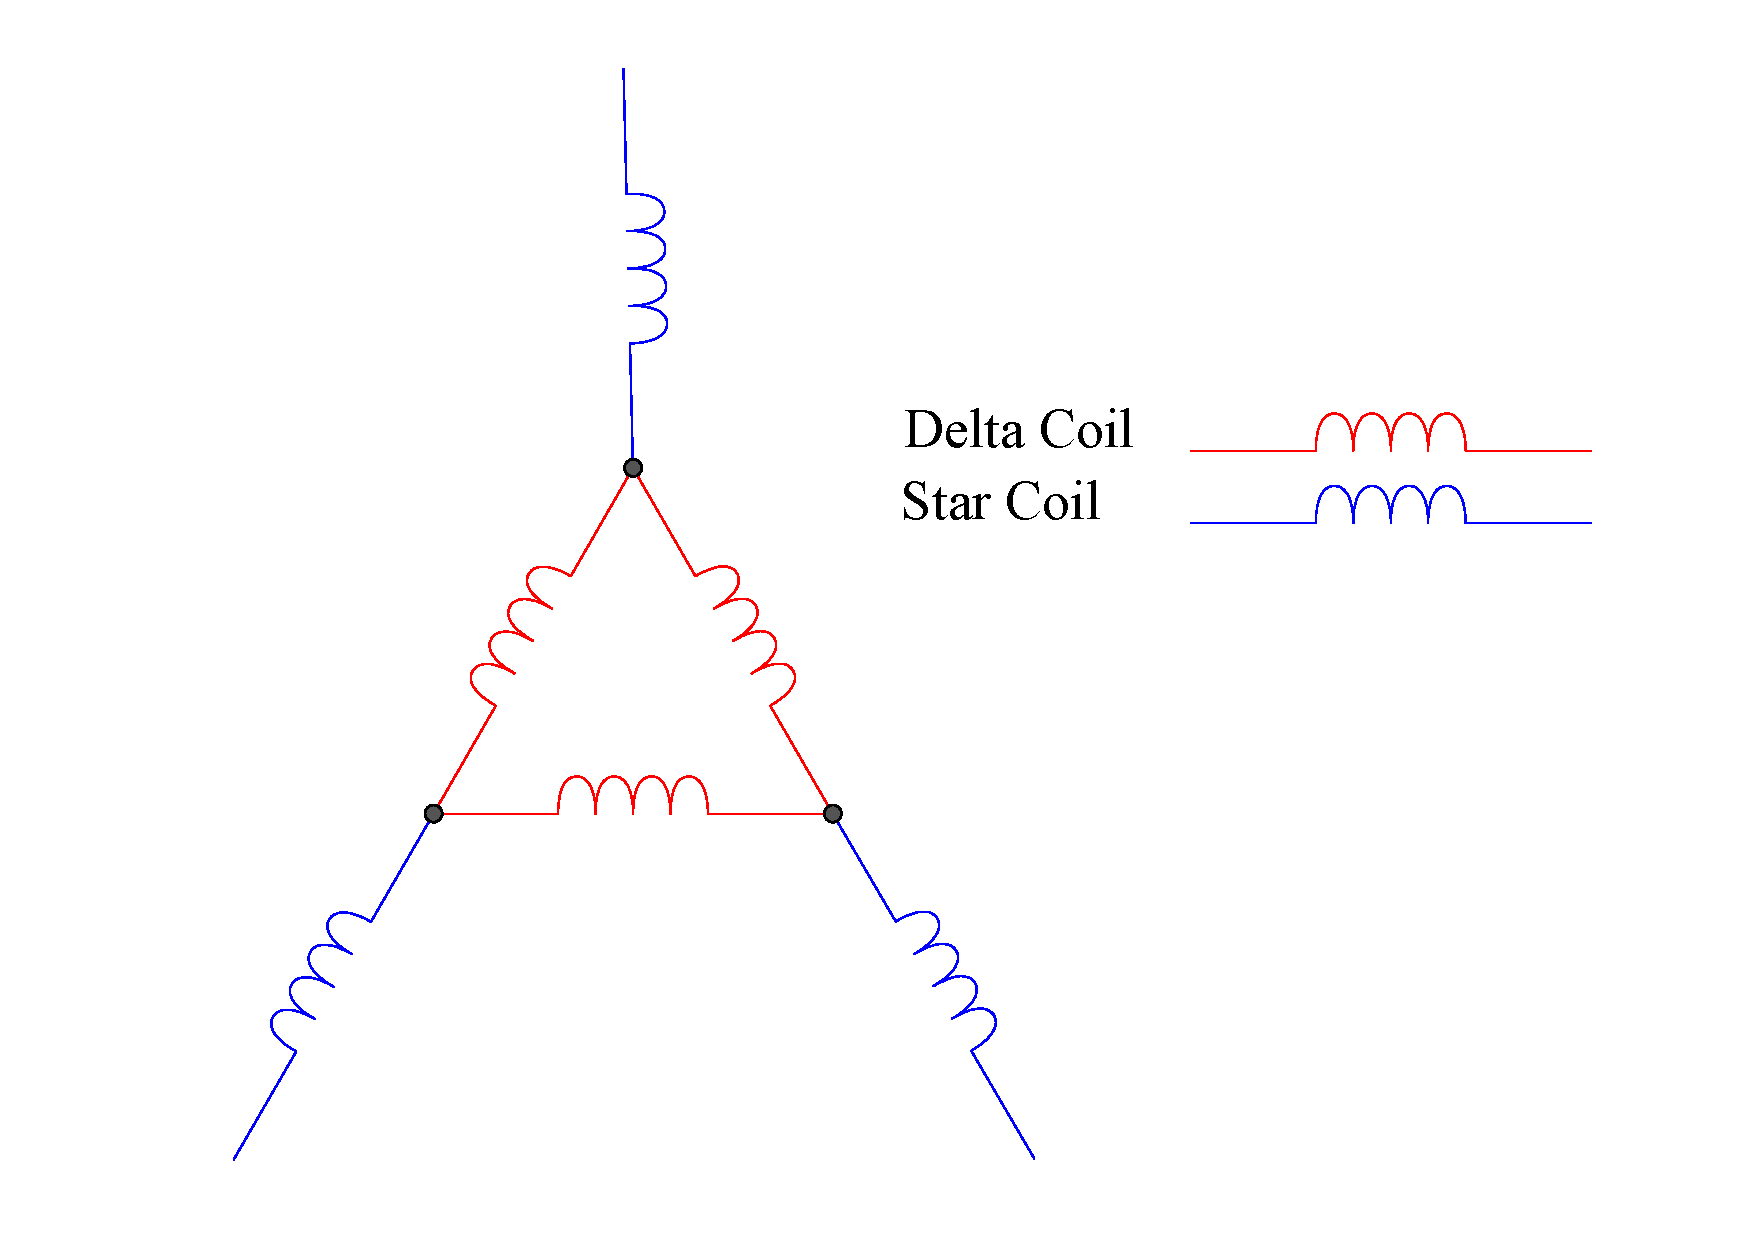
\includegraphics[width=0.7\textwidth]{src/pdf/hybrid-star-delta-wiring.pdf}
            \caption{Hybrid Star-Delta wiring of \gls{abbreviation:pmsynrelm}.}
            \label{fig:hybrid-star-delta-wiring}
        \end{figure}

        In \cite{ibrahim-permanent-magnet-assisted-synchronous-reluctance-motor-employing-a-hybrid-star-delta-winding-for-high-speed-applicaitons} the authors manufactured and proposed four prototypes of \gls{abbreviation:synrelm}. The prototypes consist of two stators, with either conventional star winding or hybrid Star-Delta winding, and two rotors, with ferrite permanent magnets or without. Maxwell transient simulations were carried out on the four prototypes, which were then manufactured and experimented on.\par
    According to \cite{ibrahim-permanent-magnet-assisted-synchronous-reluctance-motor-employing-a-hybrid-star-delta-winding-for-high-speed-applicaitons} the researches state, that when using the hybrid stator winding connection, the efficiency increase is rather low compared to efficiency increase when comparing \gls{abbreviation:synrelm} with and without \gls{abbreviation:pm}s, thus creating \gls{abbreviation:pmsynrelm}. This outcome raises a question: Is the utilization of the hybrid Star-Delta winding truly worthwhile?\par

    \subsection{Rotor}
    Rotor structure of \gls{abbreviation:pmsynrelm} draws inspiration from the design of a conventional \gls{abbreviation:synrelm}, which has undergone years of evolution to achieve wide range of constant power and near unity power factor. Rotor designs may be generally categorized as internal or external. In order to fulfill the requirements of power and power factor values, the target is to design the rotor with minimum inductane in the $q$ axis ($\text{L}_q$) and maximal inductance in $d$ axis ($\text{L}_d$). The saliency ratio defined in \cite{talebi-Design-of-Permanent-Magnet-Assisted-Synchronous-Reluctance-Motors-Made-Easy} as $\text{L}_d/\text{L}_q$ should be therefore maximized. The required saliency ratio may be achieved by optimizing shape, placement and number of flux bariers. The bariers are in \gls{abbreviation:pmsynrelm} filled with an appropriate amount of \gls{abbreviation:pm}s made of rare earth materials or ferrites. \cite{talebi-Design-of-Permanent-Magnet-Assisted-Synchronous-Reluctance-Motors-Made-Easy}\par
    In \cite{talebi-Design-of-Permanent-Magnet-Assisted-Synchronous-Reluctance-Motors-Made-Easy} authors present mathematical model of \gls{abbreviation:pmsynrelm} with four flux barriers used to propperly calculate the motor flux density, inductances, back-\gls{abbreviation:emf} and developed torque. The proposed rotor design is presented in Fig. \ref{fig:four-barrier-pmasyrelm}. There are not many papers available regarding the external rotor design of \gls{abbreviation:pmsynrelm} structure. The authors of \cite{bonthu-Design-of-permanent-magnet-assisted-synchronous-reluctance-motor-with-external-rotor-architecture} investigated the rotor structures and compared the internal and external architecture. The two compared designs are depicted in Fig. \ref{fig:external-internal-rotor}. Usually the magnetic flux density and motor parameters are analysed using Finite Element Method. The graphical analysis of the proposed four-pole \gls{abbreviation:pmsynrelm} from \cite{talebi-Design-of-Permanent-Magnet-Assisted-Synchronous-Reluctance-Motors-Made-Easy} is depicted in Fig. \ref{fig:four-pole-rotor-fem}.


    \begin{minipage}[t]{0.45\textwidth}
        \begin{figure}[H]
            \centering
            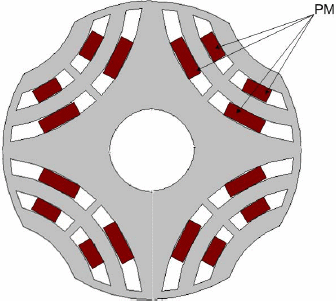
\includegraphics[width=0.95\textwidth]{src/png/four-barrier-pmasyrelm.png}
            \caption{Four barrier Permanent Magnet Assisted Synchronous Reluctance Motor rotor structure. \cite{talebi-Design-of-Permanent-Magnet-Assisted-Synchronous-Reluctance-Motors-Made-Easy}}
            \label{fig:four-barrier-pmasyrelm}
        \end{figure}
    \end{minipage}%
    \hfill
    \begin{minipage}[t]{0.45\textwidth}
        \begin{figure}[H]
            \centering
            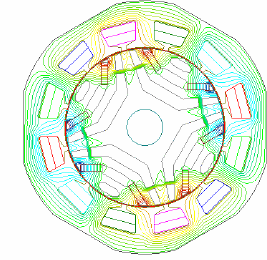
\includegraphics[width=0.85\textwidth]{src/png/four-pole-rotor-fem.png}
            \caption{Four barrier Permanent Magnet Assisted Synchronous Reluctance Motor Permanent Magnet Flux Density Analysis via Finite Element Method. \cite{talebi-Design-of-Permanent-Magnet-Assisted-Synchronous-Reluctance-Motors-Made-Easy}}
            \label{fig:four-pole-rotor-fem}
        \end{figure}
    \end{minipage}%

    \begin{figure}[htbp!]
            \centering
            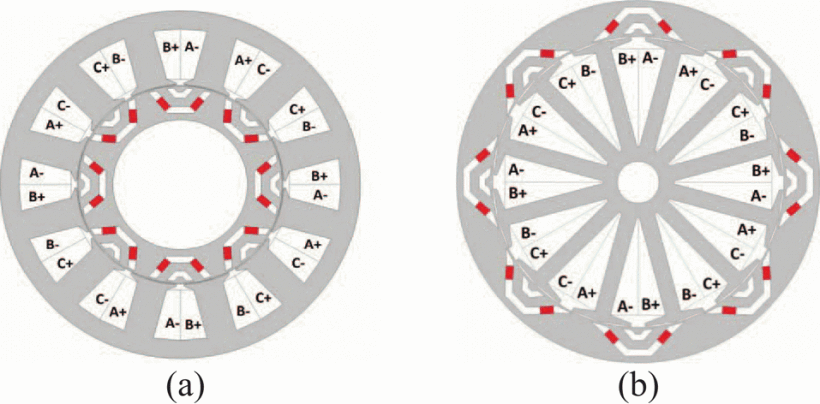
\includegraphics[width=0.8\textwidth]{src/png/external-internal-rotor.png}
            \caption{Proposed (a) internal rotor structure, (b) external rotor structure. \cite{bonthu-Design-of-permanent-magnet-assisted-synchronous-reluctance-motor-with-external-rotor-architecture}}
            \label{fig:external-internal-rotor}
    \end{figure}
    \subsubsection{Magnets}
        \gls{abbreviation:pmsynrelm} are very often compared to Permanent Magnet Synchronous Motors (\gls{abbreviation:pmsm}) in terms of power, torque density, efficiency and costs. Both of the machine types are widely used in automotive field. Though the \gls{abbreviation:pmsm} is very popular \cite{morimoto-experimental-evaulation-of-a-rare-earth-free-pmasynrm-with-ferrite-magnets-for-automotive-applications}, the permanent magnets (\gls{abbreviation:pm}s) used in the conventional design are often made of rare-earth materials such as neodymium or dysprosium. That is the motivation why \gls{abbreviation:pmsynrelm} motors with rare-earth-free materials are now being the subject of many research studies. Experiments comparing the production-used \gls{abbreviation:pmsm} and the prototype \gls{abbreviation:pmsynrelm} show, that the proposed prototype in \cite{mashiro-performance-of-mpasynrm-with-ferrite-magnets-for-ev-hv-applications-considering-productivity} achieve close values of power density and an efficiency as rare-earth \gls{abbreviation:pmsm} counterpart, but with much lower cost \cite{haiwei-low-cost-ferrite-pm-assisted-synchronous-reluctance-machine-for-electric-vehicles}.\par
It has been observed that strategically placing the \gls{abbreviation:pm}s at the center of the flux barrier forces magnetic flux lines to traverse through the flux barriers along the $q$-axis direction. This leads to reduction of a linked magnetic flux along the $q$-axis and therefore improvement of the output torque. \cite{ibrahim-permanent-magnet-assisted-synchronous-reluctance-motor-employing-a-hybrid-star-delta-winding-for-high-speed-applicaitons, ngo-performance-analysis-of-synchronous-reluctance-motor-with-limited-amount-of-permanent-magnet} The effect of \gls{abbreviation:pm} flux may be observed in a vector diagram Fig. \ref{fig:cad-pmasynrm-vector-diagram}.\par
Possible placement of \gls{abbreviation:pm}s in the rotor structure of \gls{abbreviation:pmsynrelm} is depicted in Fig. \ref{fig:pmsynrelm-rotor-magnets-position}.


    \begin{figure}[htbp!]
            \centering
            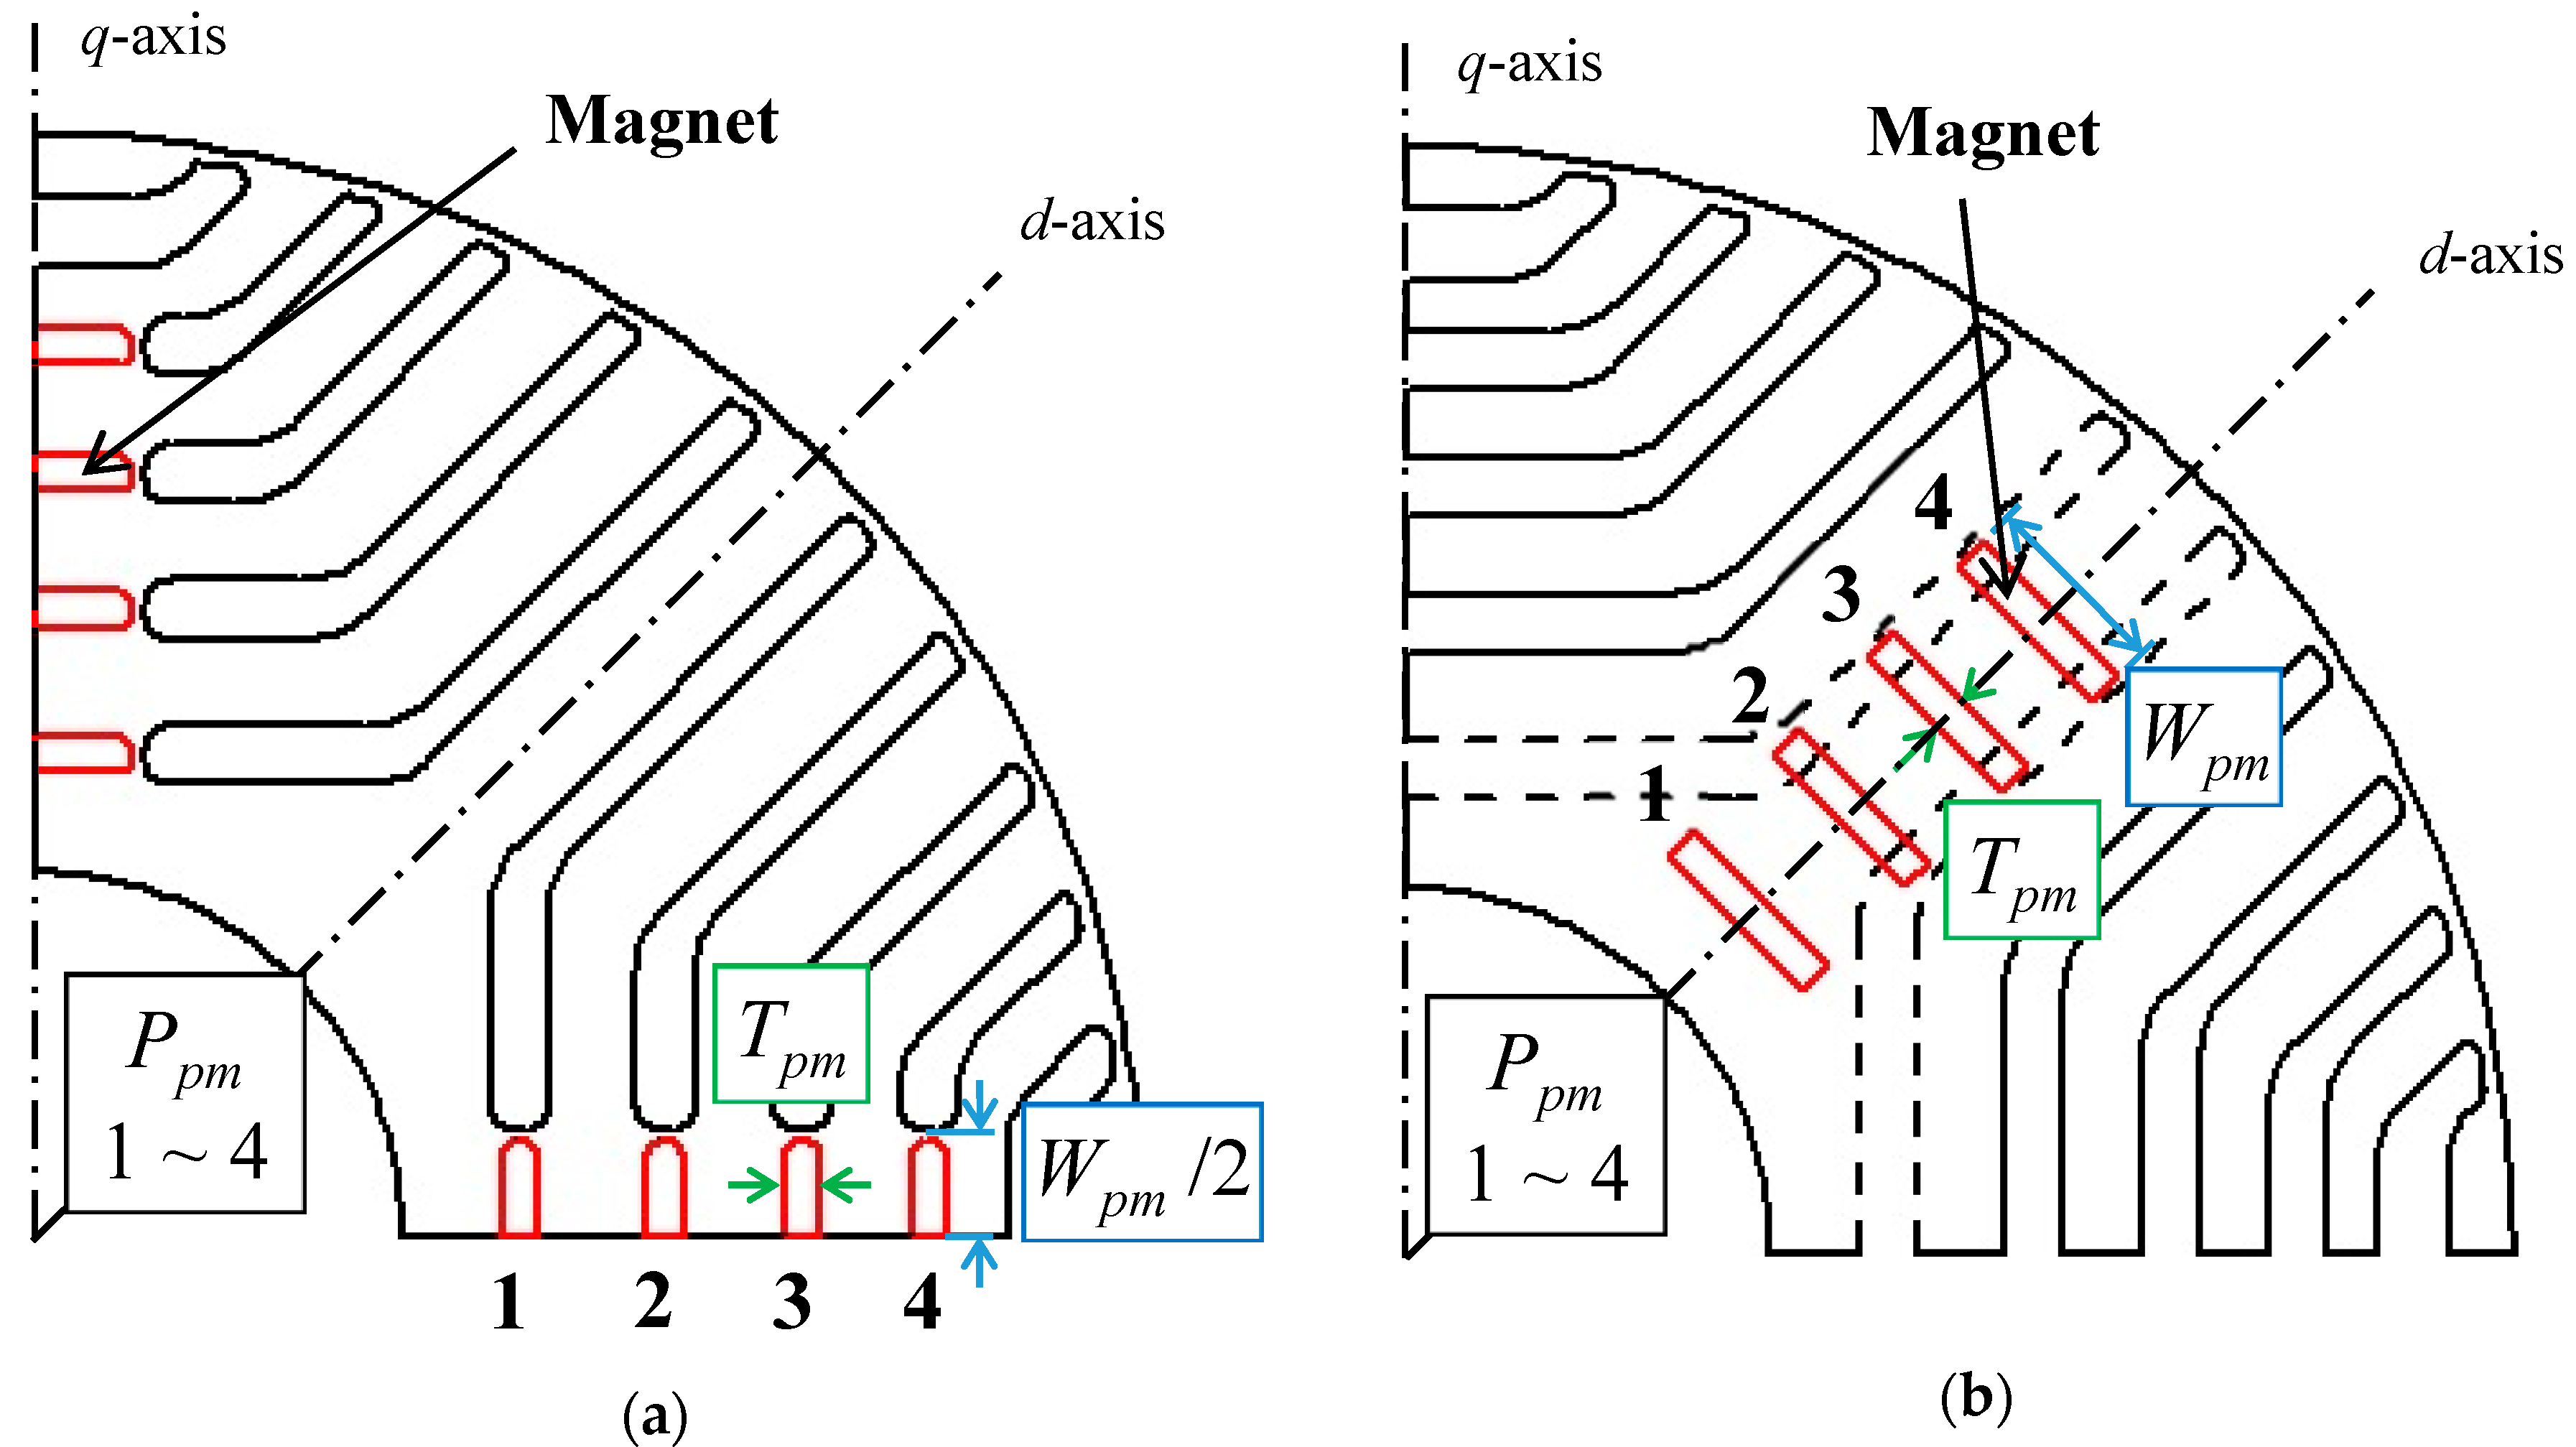
\includegraphics[width=0.8\textwidth]{src/png/pmsynrelm-rotor-magnets-position.png}
            \caption{Different approaches to a permanent magnet orientation in the rotor structure of a Permanent Magnet Assisted Synchronous Reluctance Motor. (\textbf{a}) PM embedded along the flux bariers, facing the $q$-axis; (\textbf{b}) Permanent magnets are crossing the flux bariers, therefore facing the $d$-axis. \cite{ngo-performance-analysis-of-synchronous-reluctance-motor-with-limited-amount-of-permanent-magnet}}
            \label{fig:pmsynrelm-rotor-magnets-position}
    \end{figure}

    Design of the \gls{abbreviation:pmsynrelm} rotor with \gls{abbreviation:pm}s oriented solely in the $q$-axis is depicted in the Fig. \ref{fig:pmsynrelm-rotor-magnets-q-axis}. The proces of inserting the permanent magnets to the flux barriers in the rotor is depicted in Fig. \ref{fig:pm-inserted}.
    

\begin{figure}[H]
    \begin{subfigure}{0.4\textwidth}
            \centering
            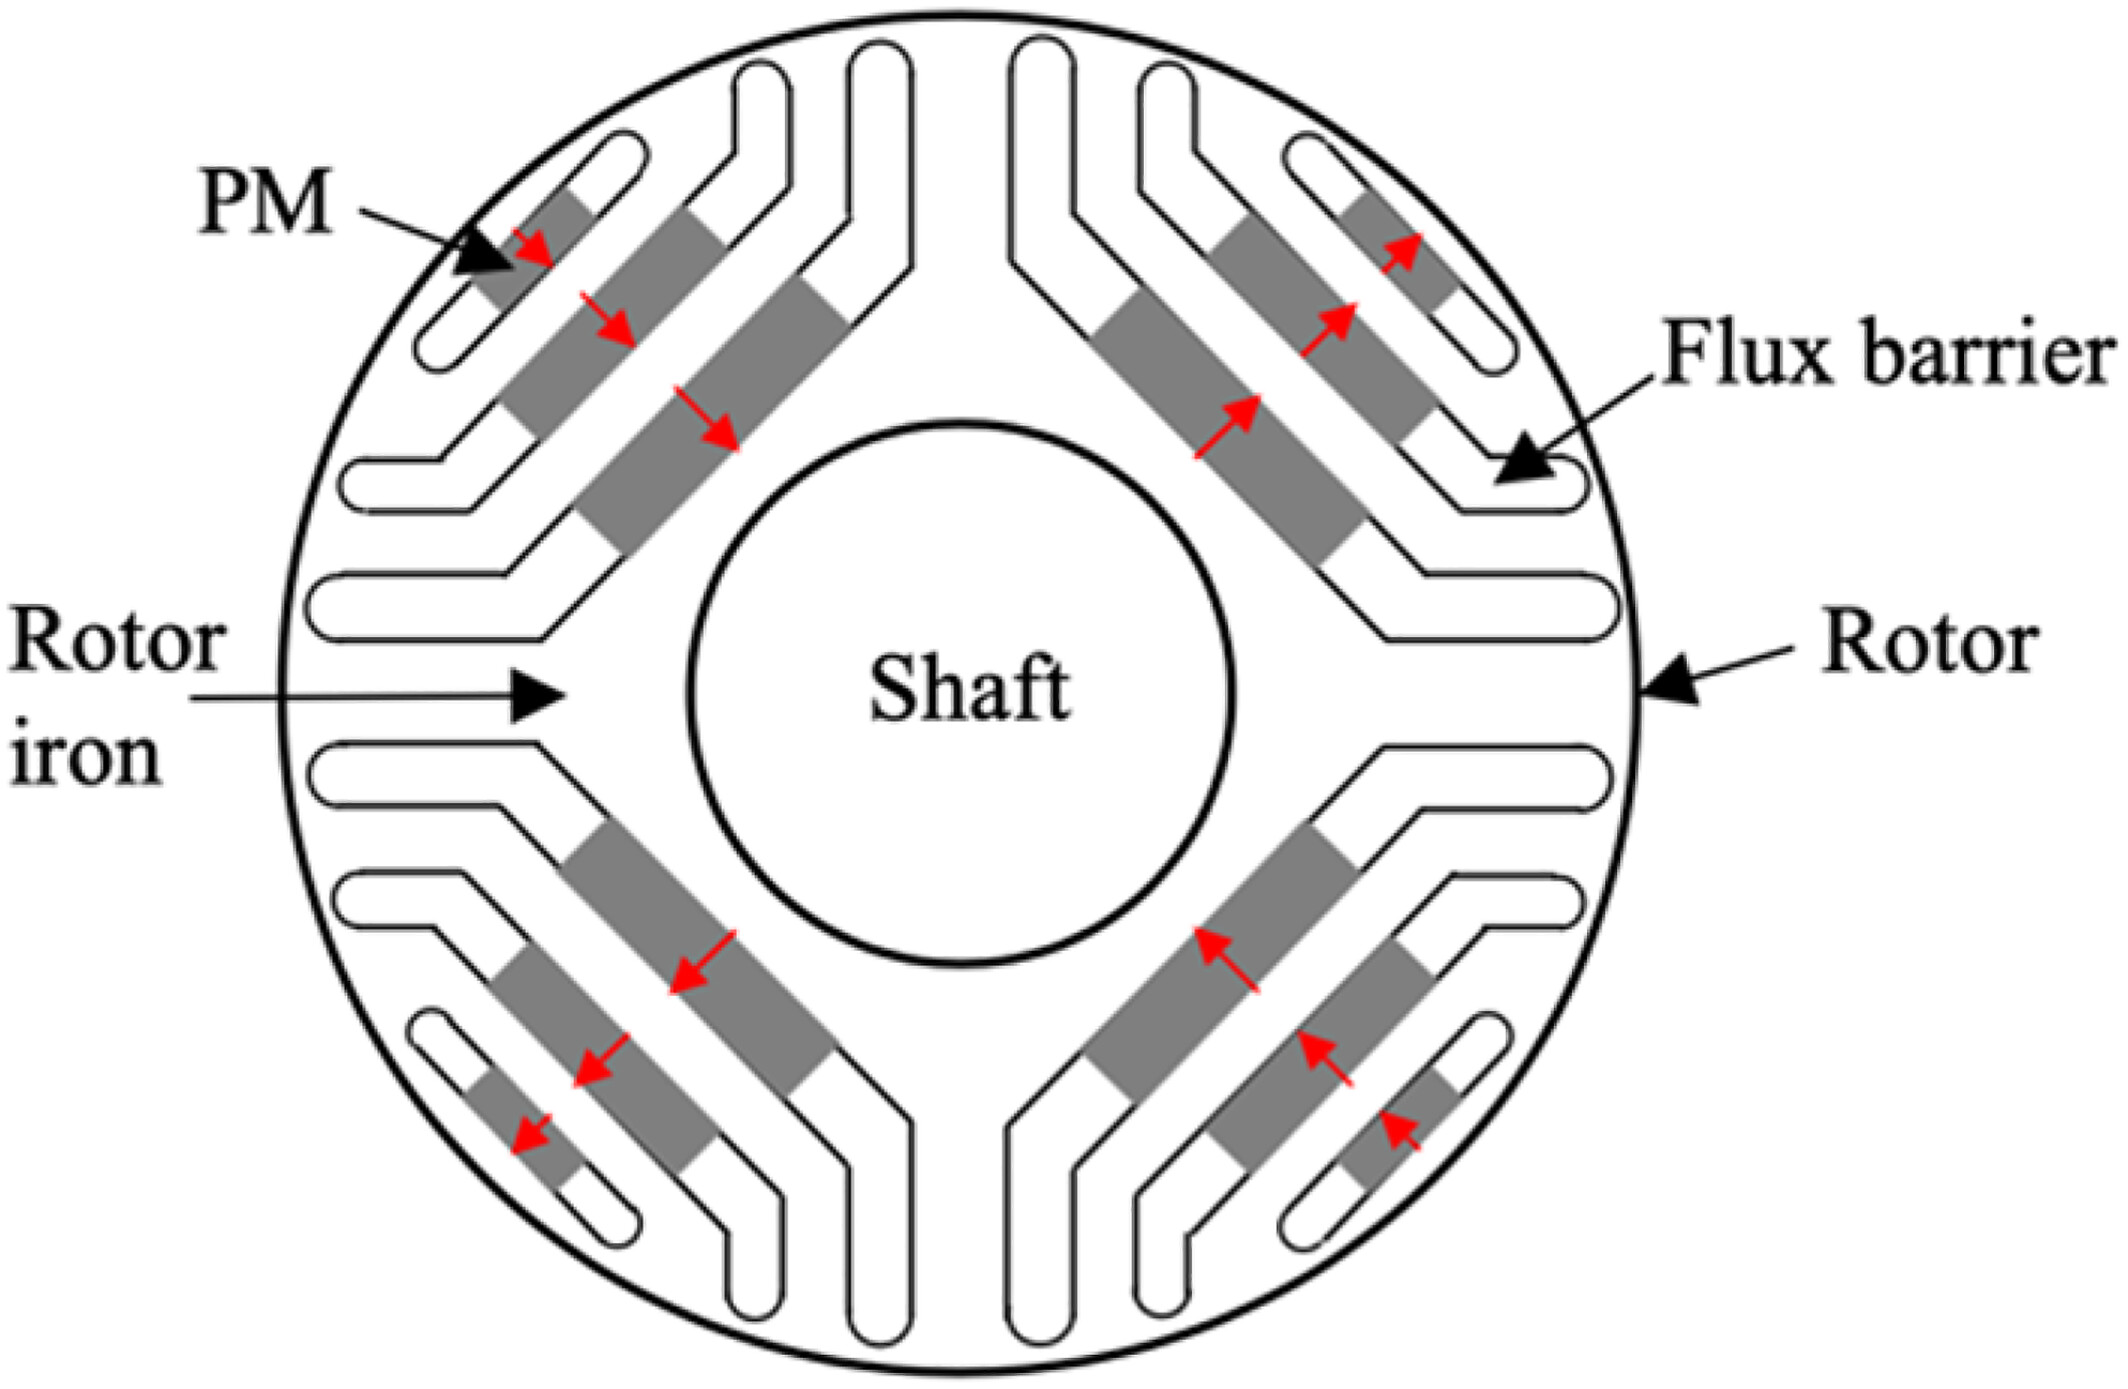
\includegraphics[width=1\textwidth]{src/png/pmsynrelm-rotor-magnets-q-axis.png}
            \caption{Rotor design of a Permanent Magnet Assisted Synchronous Reluctance Motor with permanent magnets oriented solely in the $q$-axis. \cite{tavernini-design-and-optimisation-of-energy-efficient-pmsynrelm-for-electric-vehicles}}
            \label{fig:pmsynrelm-rotor-magnets-q-axis}
    \end{subfigure}
\hfill
    \begin{subfigure}{0.4\textwidth}
            \centering
            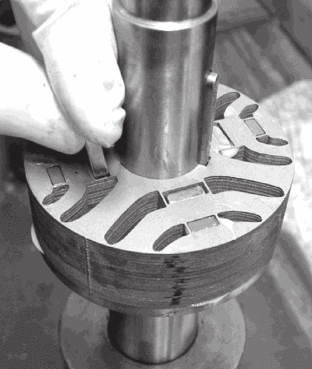
\includegraphics[width=1\textwidth]{src/png/pm-inserted.png}
            \caption{Process of inserting the permanent magnets to the rotor of a Permanent Magnet Assisted Synchronous Reluctance Motor. \cite{wang-synchronous-motors-for-traction-applications}}
            \label{fig:pm-inserted}
    \end{subfigure}
    \caption{Position of permanent magnets in a rotor design.}
\end{figure}

\FloatBarrier

%% THIS IS A NEW PART FOR ULOHA2 PART 2
\subsubsection{Effects of permanent magnet positioning on motor performance}
Authors in \cite{ngo-performance-analysis-of-synchronous-reluctance-motor-with-limited-amount-of-permanent-magnet} studied effects of various \gls{abbreviation:pm} positioning on the torque performance, torque-speed curves and demagnetization. The analysed rotor structures are depicted in the Fig. \ref{fig:pm-positioning-analysed-motor-types}.
    \begin{figure}[H]
            \centering
            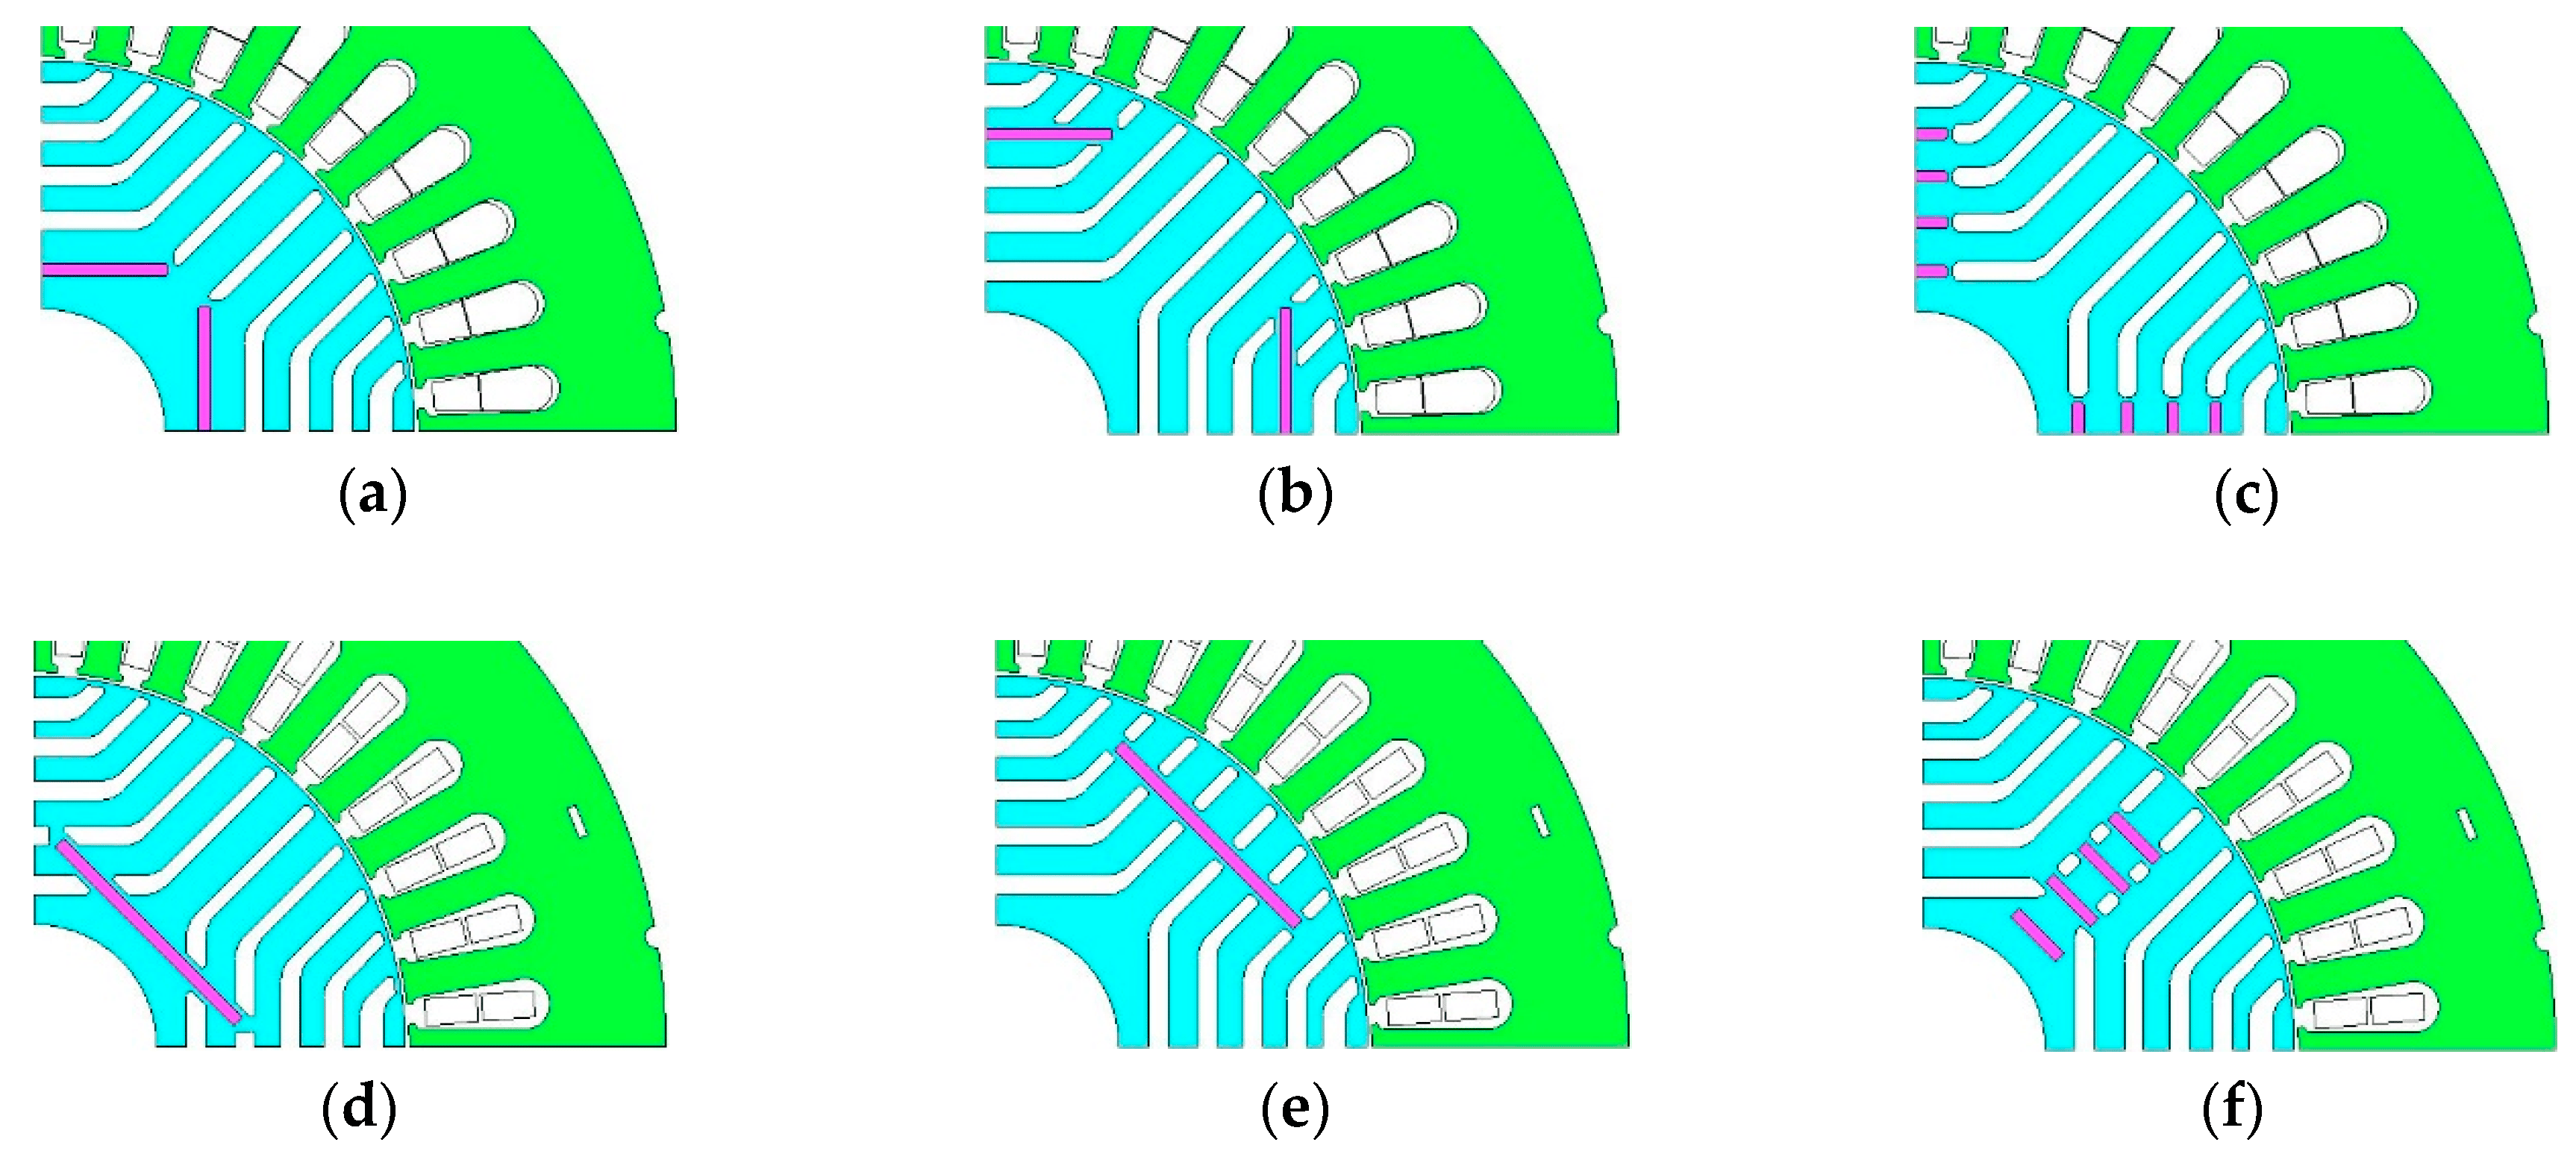
\includegraphics[width=1\textwidth]{src/png/pm-positioning-analysed-motor-types.png}
            \caption{Analysed rotor structures. \cite{ngo-performance-analysis-of-synchronous-reluctance-motor-with-limited-amount-of-permanent-magnet}}
            \label{fig:pm-positioning-analysed-motor-types}
    \end{figure}
    The authors state, that the \gls{abbreviation:pm} position has a impact on inductances of the machine which apart from stator inductances consider \gls{abbreviation:pm} flux, thus named $L_{\text{dm}}$ and $L_{\text{qm}}$. The \gls{abbreviation:pm} position in models (d), (e), (f) has a great impact on the $L_{\text{dm}}$. The lowest inductance may be observed for model (e) because of the \gls{abbreviation:pm} flux which limits the armature flux linkeage. The inductance $L_{\text{qm}}$ is by authors similar for models (d), (e), (f). The inductance $L_{\text{dm}}$ is the highest for model (c). In \cite{ngo-performance-analysis-of-synchronous-reluctance-motor-with-limited-amount-of-permanent-magnet} the authors also investigated the effect of a stator current magnitude on the inductance in.\par
    While the authors were investigating the effects on torque they found out that the torque for models (a), (b), (c) is almost similar. From the presented models, the model (c) and (a) achieve the highest torque values for the same stator current amplitude. This statement is confirmed by models.\par
    The figures Fig. \ref{fig:pm-positioning-torque-speed-curves} and Fig. \ref{fig:pm-positioning-torque-speed-curves-2} depict a torque-speed and power-speed curves of analysed rotor structures for models (c) and (a) from the preceeding figure. (named as Model 3 and Model 1 respectively) As can be seen the curves tend to converge and overlap at higher speed values. The torque and power values for the model (a) are slightly lower in the whole analysed speed range. When comparing the model (c) and (e) at the low speed operation, the torque of model (e) is still higher but when the speed increases, thus the stator current decreases because of field weakening, the power-speed curves for model (e) are enhanced. But when the speed increses and stator current still decreases, the model (e) cannot maintain its superiority and curves of model (c) surpass the (e) curves. \cite{ngo-performance-analysis-of-synchronous-reluctance-motor-with-limited-amount-of-permanent-magnet}
    From the previous conclusions it can be determined, that the specific operation point must be analyzed for the best \gls{abbreviation:pm} to be determined. In some operating points the partial shift of \gls{abbreviation:pm}s position to the $d$-axis may increase the power performance and constant power speed range of the machine.

    \begin{figure}[htbp!]
            \centering
            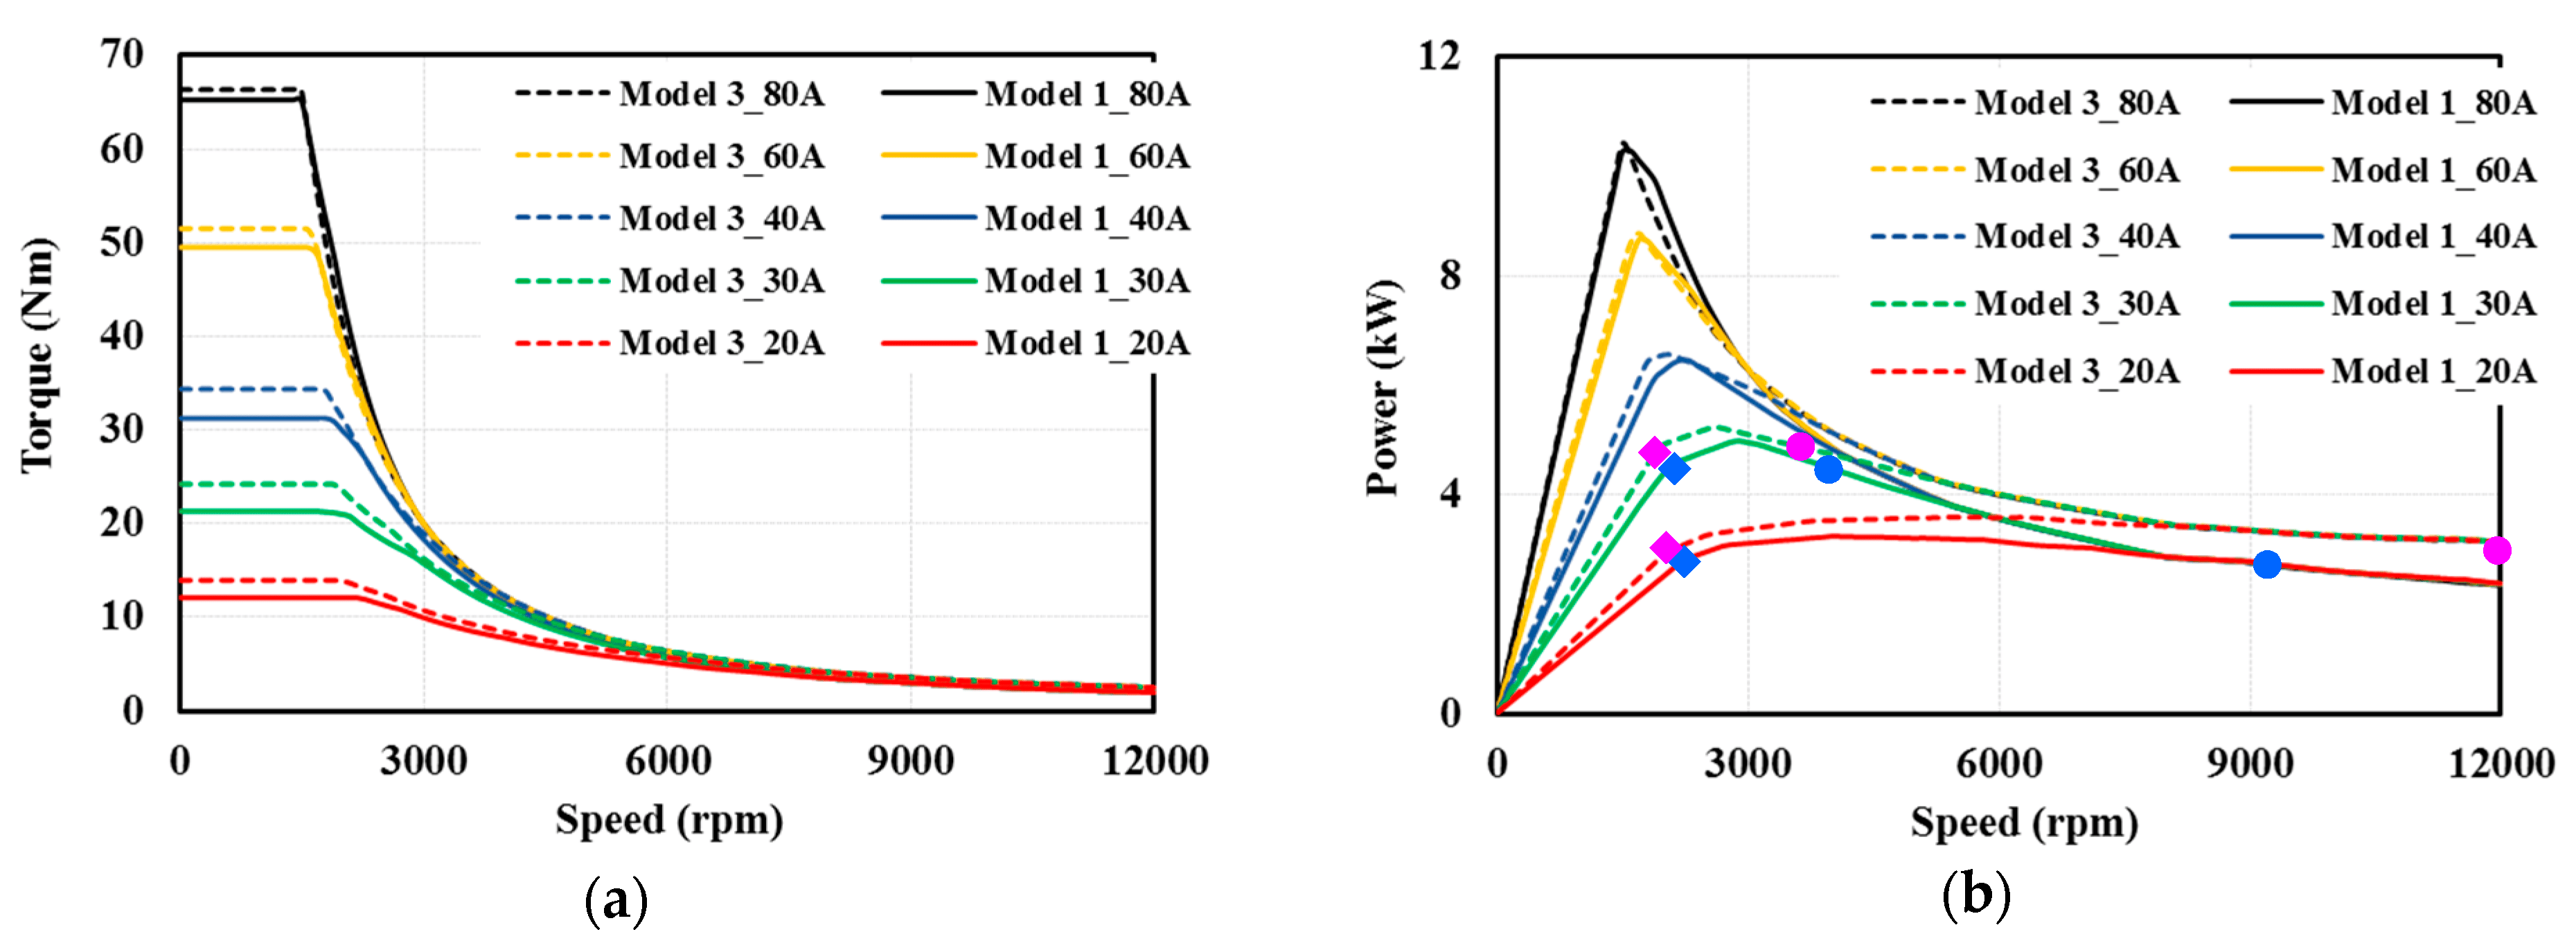
\includegraphics[width=1\textwidth]{src/png/pm-positioning-torque-speed-curves.png}
            \caption{Analysed torque-speed and power-speed curves of presented rotor structures (a) and (c) with different stator currents. \cite{ngo-performance-analysis-of-synchronous-reluctance-motor-with-limited-amount-of-permanent-magnet}}
            \label{fig:pm-positioning-torque-speed-curves}
    \end{figure}

    \begin{figure}[htbp!]
            \centering
            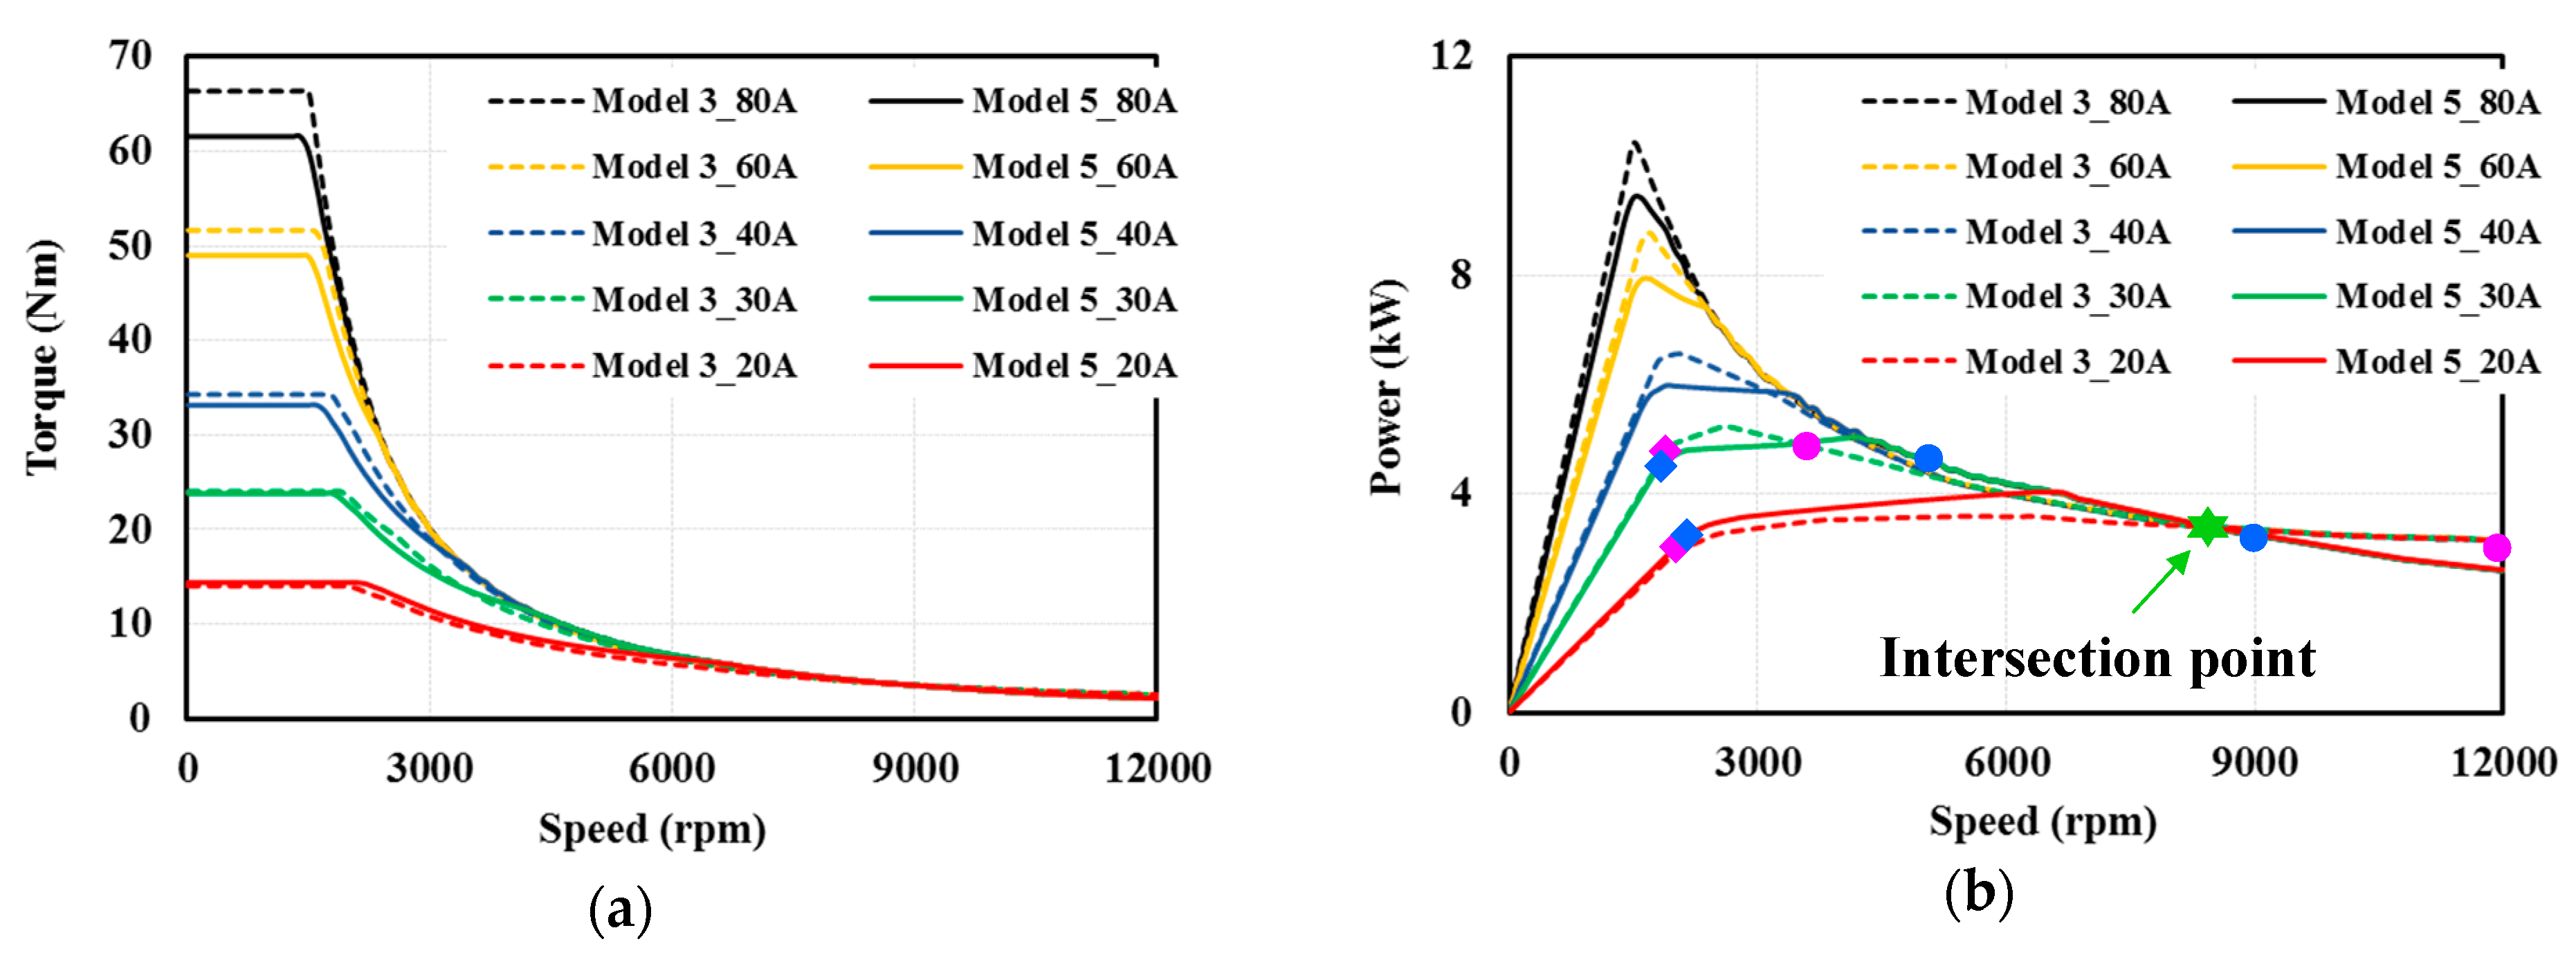
\includegraphics[width=1\textwidth]{src/png/pm-positioning-torque-speed-curves-2.png}
            \caption{Analysed torque-speed and power-speed curves of presented rotor structures (c) and (e) with different stator currents. \cite{ngo-performance-analysis-of-synchronous-reluctance-motor-with-limited-amount-of-permanent-magnet}}
            \label{fig:pm-positioning-torque-speed-curves-2}
    \end{figure}

\subsubsection{Effects of flux barrier shape on torque ripple}


    Authors in \cite{bianchi-Experimental-comparison-of-PM-assisted-synchronous-reluctance-motors} present various strategies on how to reduce the torque ripple in \gls{abbreviation:pmsynrelm}. One possibility how to reduce the ripple is to utilize the asymmetric rotor flux barriers. To compensate the ripple caused by the torque harmonics the flux barriers are slightly shifted or they adopt two different geometries in the same rotor structure. The resulting rotor structure is by authors refered to as a "machaon" type.\par
    One type of presented "machaon" rotor structure is depicted in Fig. \ref{fig:asymmetrical-rotor-flux-barriers} (c).\par
    The position of \gls{abbreviation:pm}s in the flux barrier is the same for all corresponding sections of the rotor structure, only the lateral part of barriers and ending angles differ. The small modifications of the design have impact on torque harmonics which are higher than fundamental. Thus only small variations in design are needed to inflict a change in the torque ripple. \cite{bianchi-Experimental-comparison-of-PM-assisted-synchronous-reluctance-motors}\par
    \begin{minipage}[t]{0.45\textwidth}
        \begin{figure}[H]
            \centering
            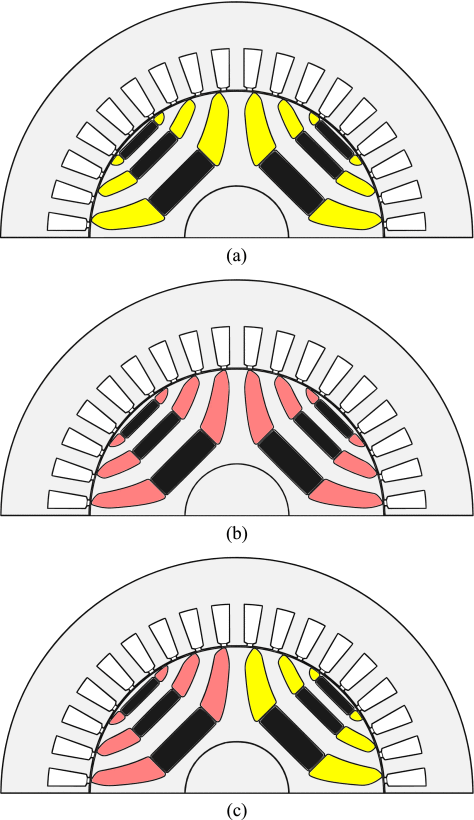
\includegraphics[width=0.85\textwidth]{src/png/asymmetrical-rotor-flux-barriers.png}
            \caption{Different geometries of rotors, symmetric type A~(a), symmetric type B (b), asymmetric (c). \cite{bianchi-Experimental-comparison-of-PM-assisted-synchronous-reluctance-motors}}
            \label{fig:asymmetrical-rotor-flux-barriers}
        \end{figure}
    \end{minipage}%
    \hspace{0.05\linewidth}
    \begin{minipage}[t]{0.45\textwidth}
        \begin{figure}[H]
            \centering
            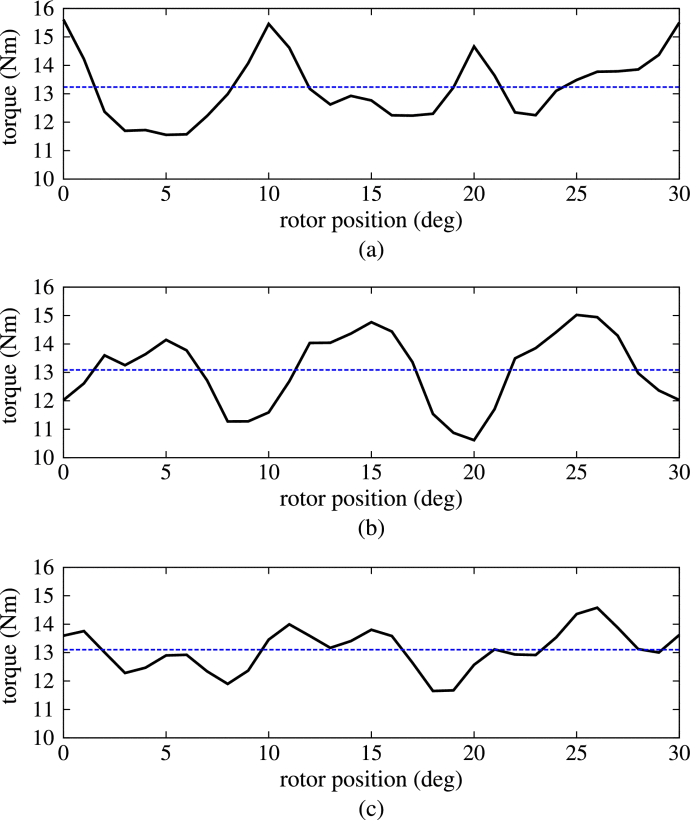
\includegraphics[width=1\textwidth]{src/png/torque-rotor-position-asymmetric-motor.png}
            \caption{Torque behaviour of symmetric A~(a), symmetric B (b) and asymmetric (c) rotors dependent on the rotor angle. \cite{bianchi-Experimental-comparison-of-PM-assisted-synchronous-reluctance-motors}}
            \label{fig:torque-rotor-position-asymmetric-motor}
        \end{figure}
    \end{minipage}%
    \FloatBarrier
    
    \vspace*{0.75cm}
    According to the \cite{bianchi-Experimental-comparison-of-PM-assisted-synchronous-reluctance-motors} authors, both of the motors with symmetric rotors from Fig. \ref{fig:asymmetrical-rotor-flux-barriers} exhibit torque harmonics of 18th order with almost the same amplitude but shifted nearly for $\pi$ radians. So when the structures are combined, the "machaon" rotor type is achieved and the 18th torque harmonics is seamingly removed. However the 36th order torque harmonics with lower amplitude caused by the torque combination of symmetric rotor types is then more evident. The authors state that the average torque value exhibits minimal variation and remains nearly same for every rotor angle position. The torque-rotor position dependency chart for symmetric rotor type~A~(a), symmetric rotor type~B~(b) and asymmetric rotor type~(c) is depicted in Fig. \ref{fig:torque-rotor-position-asymmetric-motor}.

    \par
    Numerous research studies were conducted to investigate and minimize the torque ripple. Authors of~\cite{sanada-Torque-ripple-improvement-for-synchronous-reluctance-motor-using-asymmetric-flux-barrier-arrangement} in their paper present photographs of experimental machines which were used to analyze the effects of usage of an asymmetric rotor on torque ripple. The photographs are depicted in Fig. \ref{fig:asymmetrical-rotor-experimental-photos}.

        \begin{figure}[htbp!]
            \centering
            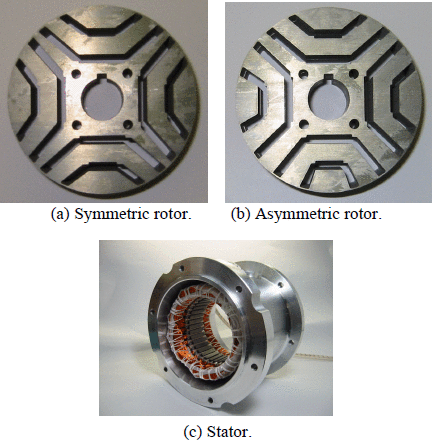
\includegraphics[width=0.55\textwidth]{src/png/asymmetrical-rotor-experimental-photos.png}
            \caption{Photographs of experimental symmetric (a) and asymmetric (b) rotor structures used by authors of \cite{sanada-Torque-ripple-improvement-for-synchronous-reluctance-motor-using-asymmetric-flux-barrier-arrangement} to analyze the effects of an asymmetrical rotor structures on a torque ripple.}
            \label{fig:asymmetrical-rotor-experimental-photos}
        \end{figure}

\FloatBarrier
%\newpage
\section{Control}

    \subsection{Mathematical model}
        The stator voltage equation of \gls{abbreviation:pmsynrelm} denoted in the general axis $k$ may be written as follows

        \begin{equation}\label{eq:voltage-equation}
            \underline{u}^k_1 = \text{R}_\text{s} \underline{i}^k_1 + \frac{\dd \underline{\psi}^k_1 }{\dd t} + j \omega_k \underline{\psi}^k_1.
        \end{equation}

        Where \gls{symbol:uk1} (V) is space vector of stator voltage, \gls{symbol:rs} ($\Omega$) is stator rezistance, \gls{symbol:ik1} (A) space vector of a stator current, \gls{symbol:psik1} (Wb) space vector of a stator flux linkeage, \gls{symbol:angularSpeed} (rad $\text{s}^{-1}$) general angular speed.\par
        The voltage equation denoted in $dq$-axis is as follows

        \begin{equation}\label{eq:stator-voltage-dq}
            \underline{u}^{dq}_1 = \text{R}_\text{s} \underline{i}^{dq}_1 + \frac{\dd \underline{\psi}^{dq}_1 }{\dd t} + j \omega_1 \underline{\psi}^k_1,
        \end{equation}
        
        where \gls{symbol:electricalAngularSpeed} (rad $\text{s}^{-1}$) is electrical angular speed of a stator rotating magnetic field. When the equation eq. \ref{eq:stator-voltage-dq} is denoted in vector components and the subscript "1" for stator is omitted the equation may be rewritten as

        \begin{equation}
            \underline{u}_d = \text{R}_\text{s} i_\text{d} + \frac{\dd \psi_d}{\dd t} - \omega_1\psi_q,
        \end{equation}
        \begin{equation}
            \underline{u}_q = \text{R}_\text{s} i_\text{q} + \frac{\dd \psi_q}{\dd t} + \omega_1\psi_d.
        \end{equation}

        Equations for flux linkeages denoted in the $dq$-axis if \gls{abbreviation:pm}s and flux are embedded along the $q$-axis are

        \begin{equation}\label{eq:d-axis-flux-linkeage}
            \psi_d = \text{L}_d i_\text{d},
        \end{equation}

        \begin{equation}\label{eq:q-axis-flux-linkeage-general}
            \psi_q = \text{L}_q i_\text{q} + \psi_\text{PM}.
        \end{equation}

        Where \gls{symbol:lq} (H), \gls{symbol:ld} (H) are inductances in $d$-axis and $q$-axis respectively, \gls{symbol:psiPM} (Wb) is a flux linkeage of permanent magnets. Very often the \gls{abbreviation:pm} flux linkeage is oriented negatively in the $q$-axis when respecting the vector orientation the equation \ref{eq:q-axis-flux-linkeage-general} can be rewritten as

        \begin{equation}\label{eq:q-axis-flux-linkeage-rewritten}
            \psi_q = \text{L}_q i_\text{q} - \psi_\text{PM}.
        \end{equation}
        
        The general equation for electromagnetic torque \gls{symbol:torque} (Nm) is then

        \begin{equation}\label{eq:torque-general}
            \begin{gathered}
                T = \frac{3}{2} \text{p}_\text{p} | \underline{\psi_{dq}} \times \underline{i_{dq}} | = \frac{3}{2} \text{p}_\text{p} (\psi_d i_q - \psi_q i_d).
            \end{gathered}
        \end{equation}

        where \gls{symbol:polePairs} (-) is number of pole pairs.\par

        After the substituion of \ref{eq:d-axis-flux-linkeage} and \ref{eq:q-axis-flux-linkeage-rewritten} to \ref{eq:torque-general} the torque euation may be rewritten as


        \begin{equation}\label{eq:torque-pmsynrelm}
            \begin{gathered}
                T = \frac{3}{2} \text{p}_\text{p} (\text{L}_d i_d i_q - (\text{L}_q i_q -\psi_\text{PM}) i_d) = \frac{3}{2} \text{p}_\text{p} (\text{L}_d i_d i_q - \text{L}_q i_q i_d + \psi_\text{PM} i_d).
            \end{gathered}
        \end{equation}

        \par
        As evident from eq. \ref{eq:torque-general}, when the linkeage flux of \gls{abbreviation:pm}s is oriented in the negative direction relative to the $q$-axis (as illustrated), an increased value of flux linkeages $\psi_\text{PM}$ results the to a higher electromagnetic torque magnitude.\par
        
        The phasor diagram is illustrated in Fig. \gls{abbreviation:synrelm} is depicted in the figure \ref{fig:cad-pmasynrm-vector-diagram}. Effect of \gls{abbreviation:pm}s layer and position in rotor on the phasor diagram may be observed in \cite{huynh-design-and-analysis-of-perm-as-synch-rel-m}.
        \begin{figure}[htbp!]
            \centering
            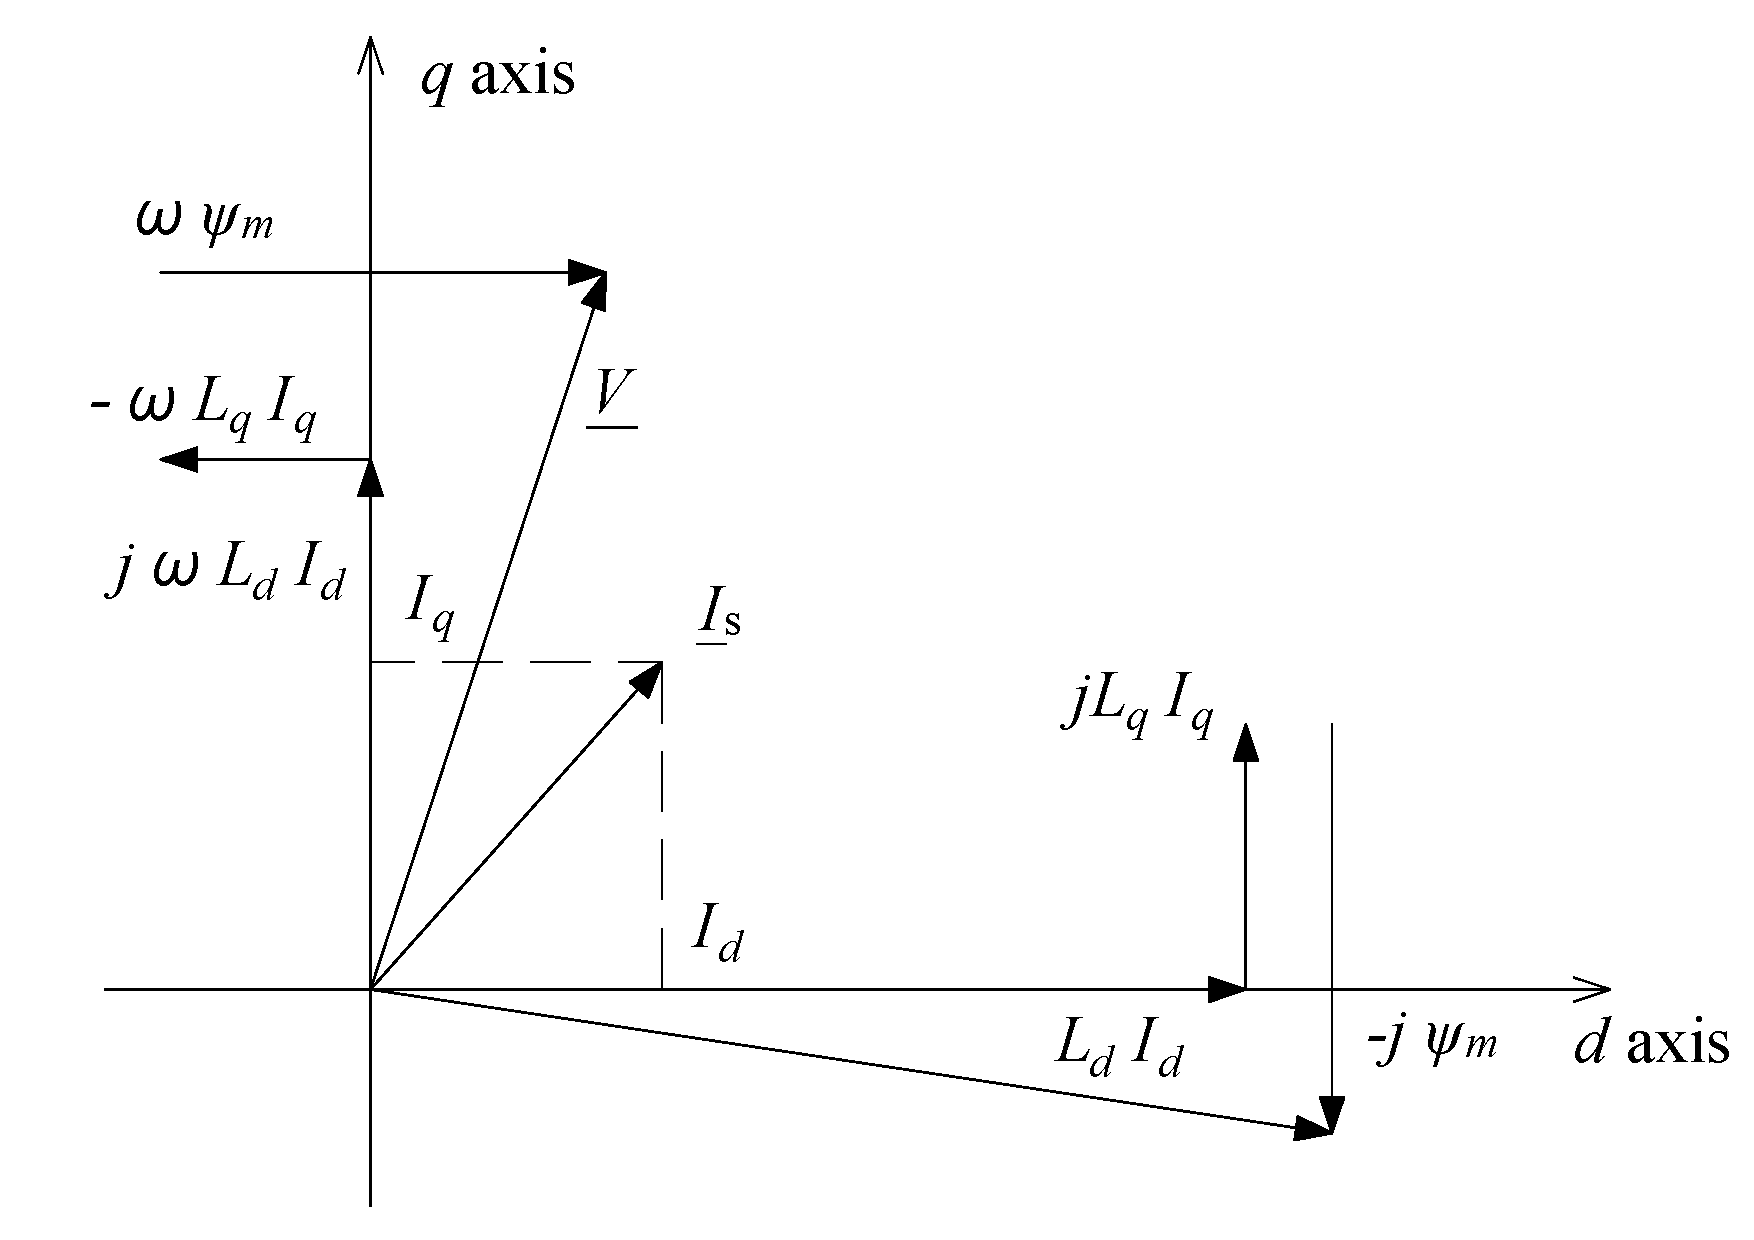
\includegraphics[width=0.70\textwidth]{src/pdf/cad-pmasynrm-vector-diagram.pdf}
            \caption{Vector diagram of the Permanent Magnet Assisted Synchronous Reluctance Motor when the flux of permanent magnets $\psi_\text{m}$ is oriented in the negative $q$-axis direction.}
            \label{fig:cad-pmasynrm-vector-diagram}
        \end{figure}
    
    \par

    When modelling the \gls{abbreviation:pmsynrelm} in simulation software such as MATLAB/Simulink it is very convinient to utilize the state-space representation of presented equations. The general \gls{abbreviation:pmsynrelm} mathematical model is presented in \cite{sriprang-Design-Modeling-and-Model-Free-Control-of-Permanent-Magnet-Assisted-Synchronous-Reluctance-Motor-for-e-Vehicle-Applications}. The state-space equations for the linkeage flux \gls{symbol:psiPM} of \gls{abbreviation:pm}s aligned with $q$-axis may be written as follows:

    \begin{equation}\label{eq:mathematical-model-pmsynrelm}
     \begin{bmatrix}
        \frac{\dd i_d}{\dd t} \\
         \frac{\dd i_q}{\dd t}
     \end{bmatrix}
        =
     \begin{bmatrix}
         - \frac{R_\mathrm{s}}{L_d}i_d + \frac{\omega_1}{L_d}(L_q i_q - \psi_\mathrm{PM})\\
         - \frac{\omega_1 L_d}{L_q} - \frac{R_s}{L_q} i_q
     \end{bmatrix}
        +
     \begin{bmatrix}
        \frac{1}{L_d} & 0\\
         0 & \frac{1}{L_q}
     \end{bmatrix}
     \begin{bmatrix}
         u_{1d}\\
         u_{1q}
     \end{bmatrix}.
    \end{equation}
    It is convinient to include the torque equation \ref{eq:torque-pmsynrelm} to the model as

    \begin{equation}
        T = \frac{3}{2} p_\mathrm{p} i_d \left[ i_q (L_d - L_q) + \psi_{\mathrm{PM}} \right].
    \end{equation}

    
    \par

    The formulation of the state-space representation primarily originates from the stator voltage equation, as expressed in Eq. \ref{eq:voltage-equation}.

    \subsection{Control strategies}

        Numerous options exist for controlling the \gls{abbreviation:pmsynrelm}. The principles may be broadly categorized into two major groups: \textbf{Scalar Control} and \textbf{Vector Control}. The primary subcategories of vector control strategies are \textbf{Field Oriented Control} (\gls{abbreviation:foc}) and \textbf{Direct Torque Control} (\gls{abbreviation:dtc}). These strategies use a different approach to minimize the torque ripple and to achive desirable high dynamic performance. \cite{dwivedi-review-on-control-strategies-of-permanent-magnet-assisted-synchronous-reluctance-motor-drive} The general group decopmosition is depicted in Fig. \ref{fig:pmsynrelm-control-strategies}.

        \begin{figure}[htbp!]
            \centering
            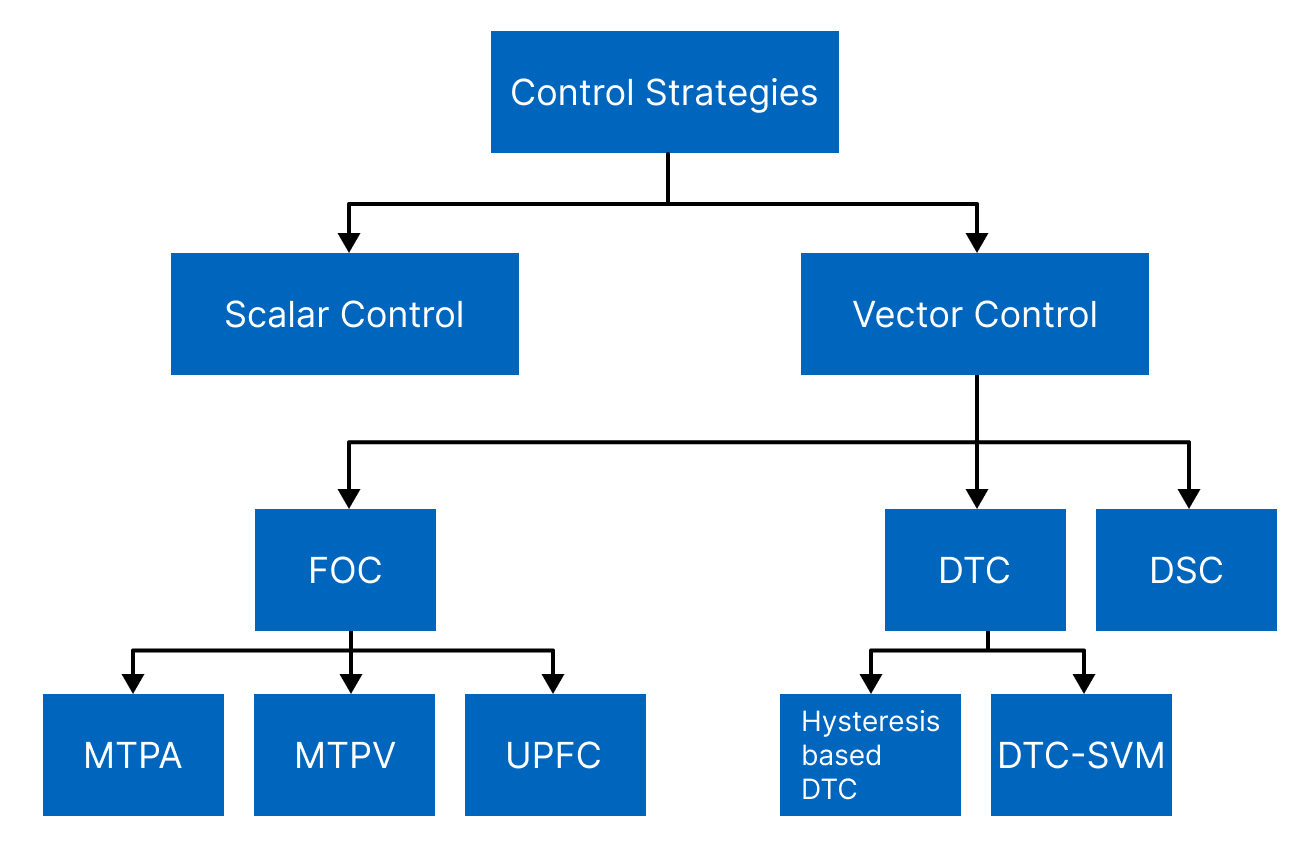
\includegraphics[width=0.75\textwidth]{src/png/pmsynrelm-control-strategies.png}
            \caption{General diagram depicting major groups of control strategies for \gls{abbreviation:pmsynrelm}. Graph inspired by \cite{dwivedi-review-on-control-strategies-of-permanent-magnet-assisted-synchronous-reluctance-motor-drive}}
            \label{fig:pmsynrelm-control-strategies}
        \end{figure}


        \subsubsection{Scalar Control}
            Executing scalar drive control is relatively straighforward solution, it does not necesitate the use of high performance Digital Signal Processors (\gls{abbreviation:dsp}s). However Scalar Control does not provide the great dynamic performance and speed provided by \gls{abbreviation:foc} and \gls{abbreviation:dtc}. \cite{dwivedi-review-on-control-strategies-of-permanent-magnet-assisted-synchronous-reluctance-motor-drive}\par
            Scalar control is mainly known as a $V$/$f$ (Voltage/frequency) control. The control methods primarily generate output voltage, maintaining a constant ratio between voltage and frequency. The ratio is kept constant for the magnetizing flux to be the highest possible, so the torque is maximized as well. Another methods may use $I$/$f$ (current/frequency) control based strategies. \cite{heidari-a-review-of-synchronour-relucatence-motor-drive-advancements}

        \subsubsection{Vector Control}
            Vector control strategies have become increasingly popular, thanks to the combination of lower cost and hightened computational power of general \gls{abbreviation:dsp}s. \cite{dwivedi-review-on-control-strategies-of-permanent-magnet-assisted-synchronous-reluctance-motor-drive}
            \par
            \gls{abbreviation:foc} mainly leverages the theory of space vectors, while \gls{abbreviation:dtc} employs the theory of controlling the electromagnetic torque and magnetic flux directly based on the reference speed and magnetic flux. \gls{abbreviation:foc} and \gls{abbreviation:dtc} strategies differ but objective remains unchanged. The primary goal of vector control strategies is to attain the desired torque and flux values based on the reference values which are set as an input to the control strategy. \cite{heidari-a-review-of-synchronour-relucatence-motor-drive-advancements, dwivedi-review-on-control-strategies-of-permanent-magnet-assisted-synchronous-reluctance-motor-drive}
            
            \vspace*{0.45cm}
             \hspace*{-\parindent} \textbf{Maximum Torque Per Ampere (\gls{abbreviation:mtpa}) \gls{abbreviation:pmsynrelm} control}\par
                \hspace*{\parindent} The main objective of the strategy is to achieve the reference torque using minimum value of stator current $i_d$ and $i_q$. According to \cite{dwivedi-review-on-control-strategies-of-permanent-magnet-assisted-synchronous-reluctance-motor-drive}, there are numerous methods how to realize the \gls{abbreviation:mtpa}.\par
                The control strategy is parameter dependent which may present a problem. In \cite{niazi-robust-maximum-torque-per-ampere-control-of-pmsynrelm} authors present a robust online parameter estimation technique which improves the general \gls{abbreviation:mtpa} control strategy. Using calculated and estimated parameters together with measured stator currents the machine torque is calculated and then used as a reference value for further calculations. The proposed controller stands out for its increased robustness againts the variations of motor parameters.
                \par
                Authors in \cite{sriprang-Design-Modeling-and-Model-Free-Control-of-Permanent-Magnet-Assisted-Synchronous-Reluctance-Motor-for-e-Vehicle-Applications} present a model-free \gls{abbreviation:mtpa} control of the \gls{abbreviation:pmsynrelm}. The motor is modelled with equations presented in this section. The authors modelled the control and motor part in MATLAB and then performed the experimentation measuring using 1 kW motor. The motor parameters are present in the cited paper. The model-free approach is best for complex systems, where the control strategies are parameter dependet or there are not enough known parameters of controlled system. Authors then conclude that their presented model-free control algorithm tracks the reference values well and is suitable for controlling the machine.In terms of performance the proposed model-free control technique surpassed the \gls{abbreviation:foc} with traditional proportional-integral controllers. Similar approach was taken to improve the control strategies for \gls{abbreviation:pmsm} \cite{wang-Modulated-Model-Free-Predictive-Control-With-Minimum-Switching-Losses-for-PMSM-Drive-System} and \gls{abbreviation:synrelm} \cite{lin-A-Modulated-Model-Free-Predictive-Current-Control-for-Four-Switch-Three-Phase-Inverter-Fed-SynRM-Drive-Systems} drives.

            \vspace*{1.5cm}
             \hspace*{-\parindent} \textbf{Maximum Torque Per Voltage (\gls{abbreviation:mtpv}) \gls{abbreviation:pmsynrelm} control}\par
                \hspace*{\parindent} The higher the rotor angular speed, the larger the magnitude of the back electromotive force (\gls{abbreviation:emf}), the larger voltage magnitude supplied from source is needed for machine to work correctly. When rotor speed reaches the value where back \gls{abbreviation:emf} is so high that the higher supply voltage than the nominal is required then the current flowing through stator wires decreases. This is due to the back \gls{abbreviation:emf} and inability to highten the supply voltage above the nominal. Thus the voltage value restricts the current based on the rotor speed. In \cite{sanz-analitical-maximum-torque-per-volt-control-strategu-of-an-interior-permanent-magnet-synchronous-motor-with-very-low-battery-voltage} the exemplar curves presenting \gls{abbreviation:mtpv} are depicted. Another mathematical expression of the \gls{abbreviation:mtpv} trajectory is presented in \cite{fletcher-operation-along-the-maximum-torque-per-voltage-trajectory-in-a-direct-torque-and-flux-controlled-interior-permament-magnet-synchronous-motor}. Cited paper also depicts the exemplar trajectories in the $i_d$-$i_q$ plane.
                \par
                The \gls{abbreviation:mtpv} trajectories are plotted in the $i_d$-$i_q$ plane. The trajectories correspond to the operation points where the possible torque is at the peak value. Thus the maximum torque value depends on the operational rotor speed.

            \newpage
            %\vspace*{1.5cm}
             \hspace*{-\parindent} \textbf{Unity Power Factor Control (\gls{abbreviation:upfc})}\par
             \hspace*{\parindent} In various applications, it is required for the machine to operate with the highest power factor possible. Achieving a unity power factor is preferable to eliminate the consumption of reactive power. In \cite{moussa-unity-power-factor-control-of-permanent-magnet-motor-drive-system} two methods for achieving the highest value of power factor are proposed: \textit{1) controlling the $d$-axis stator current $i_d$} and \textit{2) controling the angle of stator current space vector $\underline{i_\text{stator}}$}.\par
             According to \cite{moussa-unity-power-factor-control-of-permanent-magnet-motor-drive-system} the \gls{abbreviation:upfc} allows wider speed range with constant torque value. This results in a higher output power of the drive.\par

             \vspace*{0.85cm}
             \textit{1) controling the $d$-axis stator current $i_d$}\par
             \hspace*{\parindent} Method compares space angles of stator current and voltage space vectors to achieve the unity power factor. The value of the current $i_\text{d}$ which satisfies the unity power factor condition then may be expressed and passed to the stator voltage equations of \gls{abbreviation:pmsynrelm}. The equations then may be modified to evaulate the steady-state performance and required voltage space vector at a unity power-factor. \cite{moussa-unity-power-factor-control-of-permanent-magnet-motor-drive-system}

             \vspace*{0.85cm}
             \textit{2) controling the angle of stator current space vector $i_\text{stator}$}\par
             \hspace*{\parindent} This method forces the space vector of a stator current to be aligned with space vector of a stator electromagnetic force by modifying the value of the vector components. When the space vectors of a stator voltage and current will coincide the unity power factor will be achieved. \cite{moussa-unity-power-factor-control-of-permanent-magnet-motor-drive-system}

        \subsubsection{Direct Torque Control}
            Compared to vector control the \gls{abbreviation:dtc} is in fact simpler. It does not require the Pulse Width Modulation (\gls{abbreviation:pwm}) techniques. During the sample periode of \gls{abbreviation:dsp} only one space vector of supply voltage is provided as an output from the inverter. The calculation and control is done in the stationary reference frame (eg. stator linked frame in $\alpha \beta$ axis system).

            \vspace*{1.5cm}
             \hspace*{-\parindent} \textbf{Hysteresis based \gls{abbreviation:dtc}}\par
            \hspace*{\parindent} Hysteresis based \gls{abbreviation:dtc} uses the principle of keeping the values of torque and magnetic flux (independently) in the hysteresis band of allowed values. Hysteresis based \gls{abbreviation:dtc} needs only a portion of paramaters which are necessary for vector control strategies, thus making the method very elegant and convinient. \cite{dwivedi-review-on-control-strategies-of-permanent-magnet-assisted-synchronous-reluctance-motor-drive}\par


            \vspace*{0.85cm}
             \hspace*{-\parindent} \textbf{\gls{abbreviation:dtc} Space Vector Modulation (\gls{abbreviation:svm})}\par
            \hspace*{\parindent} \gls{abbreviation:dtc} Space Vector Modulation (\gls{abbreviation:svm}) utilizes general \gls{abbreviation:dtc} strategy but instead of hysteresis controllers the proportional-integral regulators with predictive controllers are used. Strategy proposed in \cite{swierczynski-dsp-based-direct-torque-control-of-permanent-magnet-synchronous-motor-using-space-vector-modulation-dtcsvm} shows that for Permanent Magnet Synchronous Motor the \gls{abbreviation:dtc}-\gls{abbreviation:svm} results in lower torque ripple and better harmonic composition of stator current than conventional \gls{abbreviation:dtc}.

        
        \newpage
        \subsubsection{Direct Self Control}
            Direct Self Control \gls{abbreviation:dsc} is very similar to the \gls{abbreviation:dtc} strategy, which was published by Takahashi in \cite{takahashi-high-performance-direct-torque-control-of-an-iduction-motor} in 1989 for induction motor. The \gls{abbreviation:dsc} strategy was published by Depenbrock in \cite{depenbrock-direct-self-control-of-inverter-fed-induction-machine}. In the proposed strategy the voltage space vectors follow the hexagonal path. In comparision \gls{abbreviation:dsc} strategy generaly requires lower switching frequency of the components than the \gls{abbreviation:dtc}.

        \subsubsection{Other strategies}
            Numerous research papers have been published regarding the control strategies which leverage the fundamental principe of the general strategies and refines them for the specific application. The example diagram depicting some popular derived strategies of general \gls{abbreviation:synrelm} is presented in Fig. \ref{fig:control-strategies-diagram} \cite{heidari-a-review-of-synchronour-relucatence-motor-drive-advancements}.

        \begin{figure}[htbp!]
            \centering
            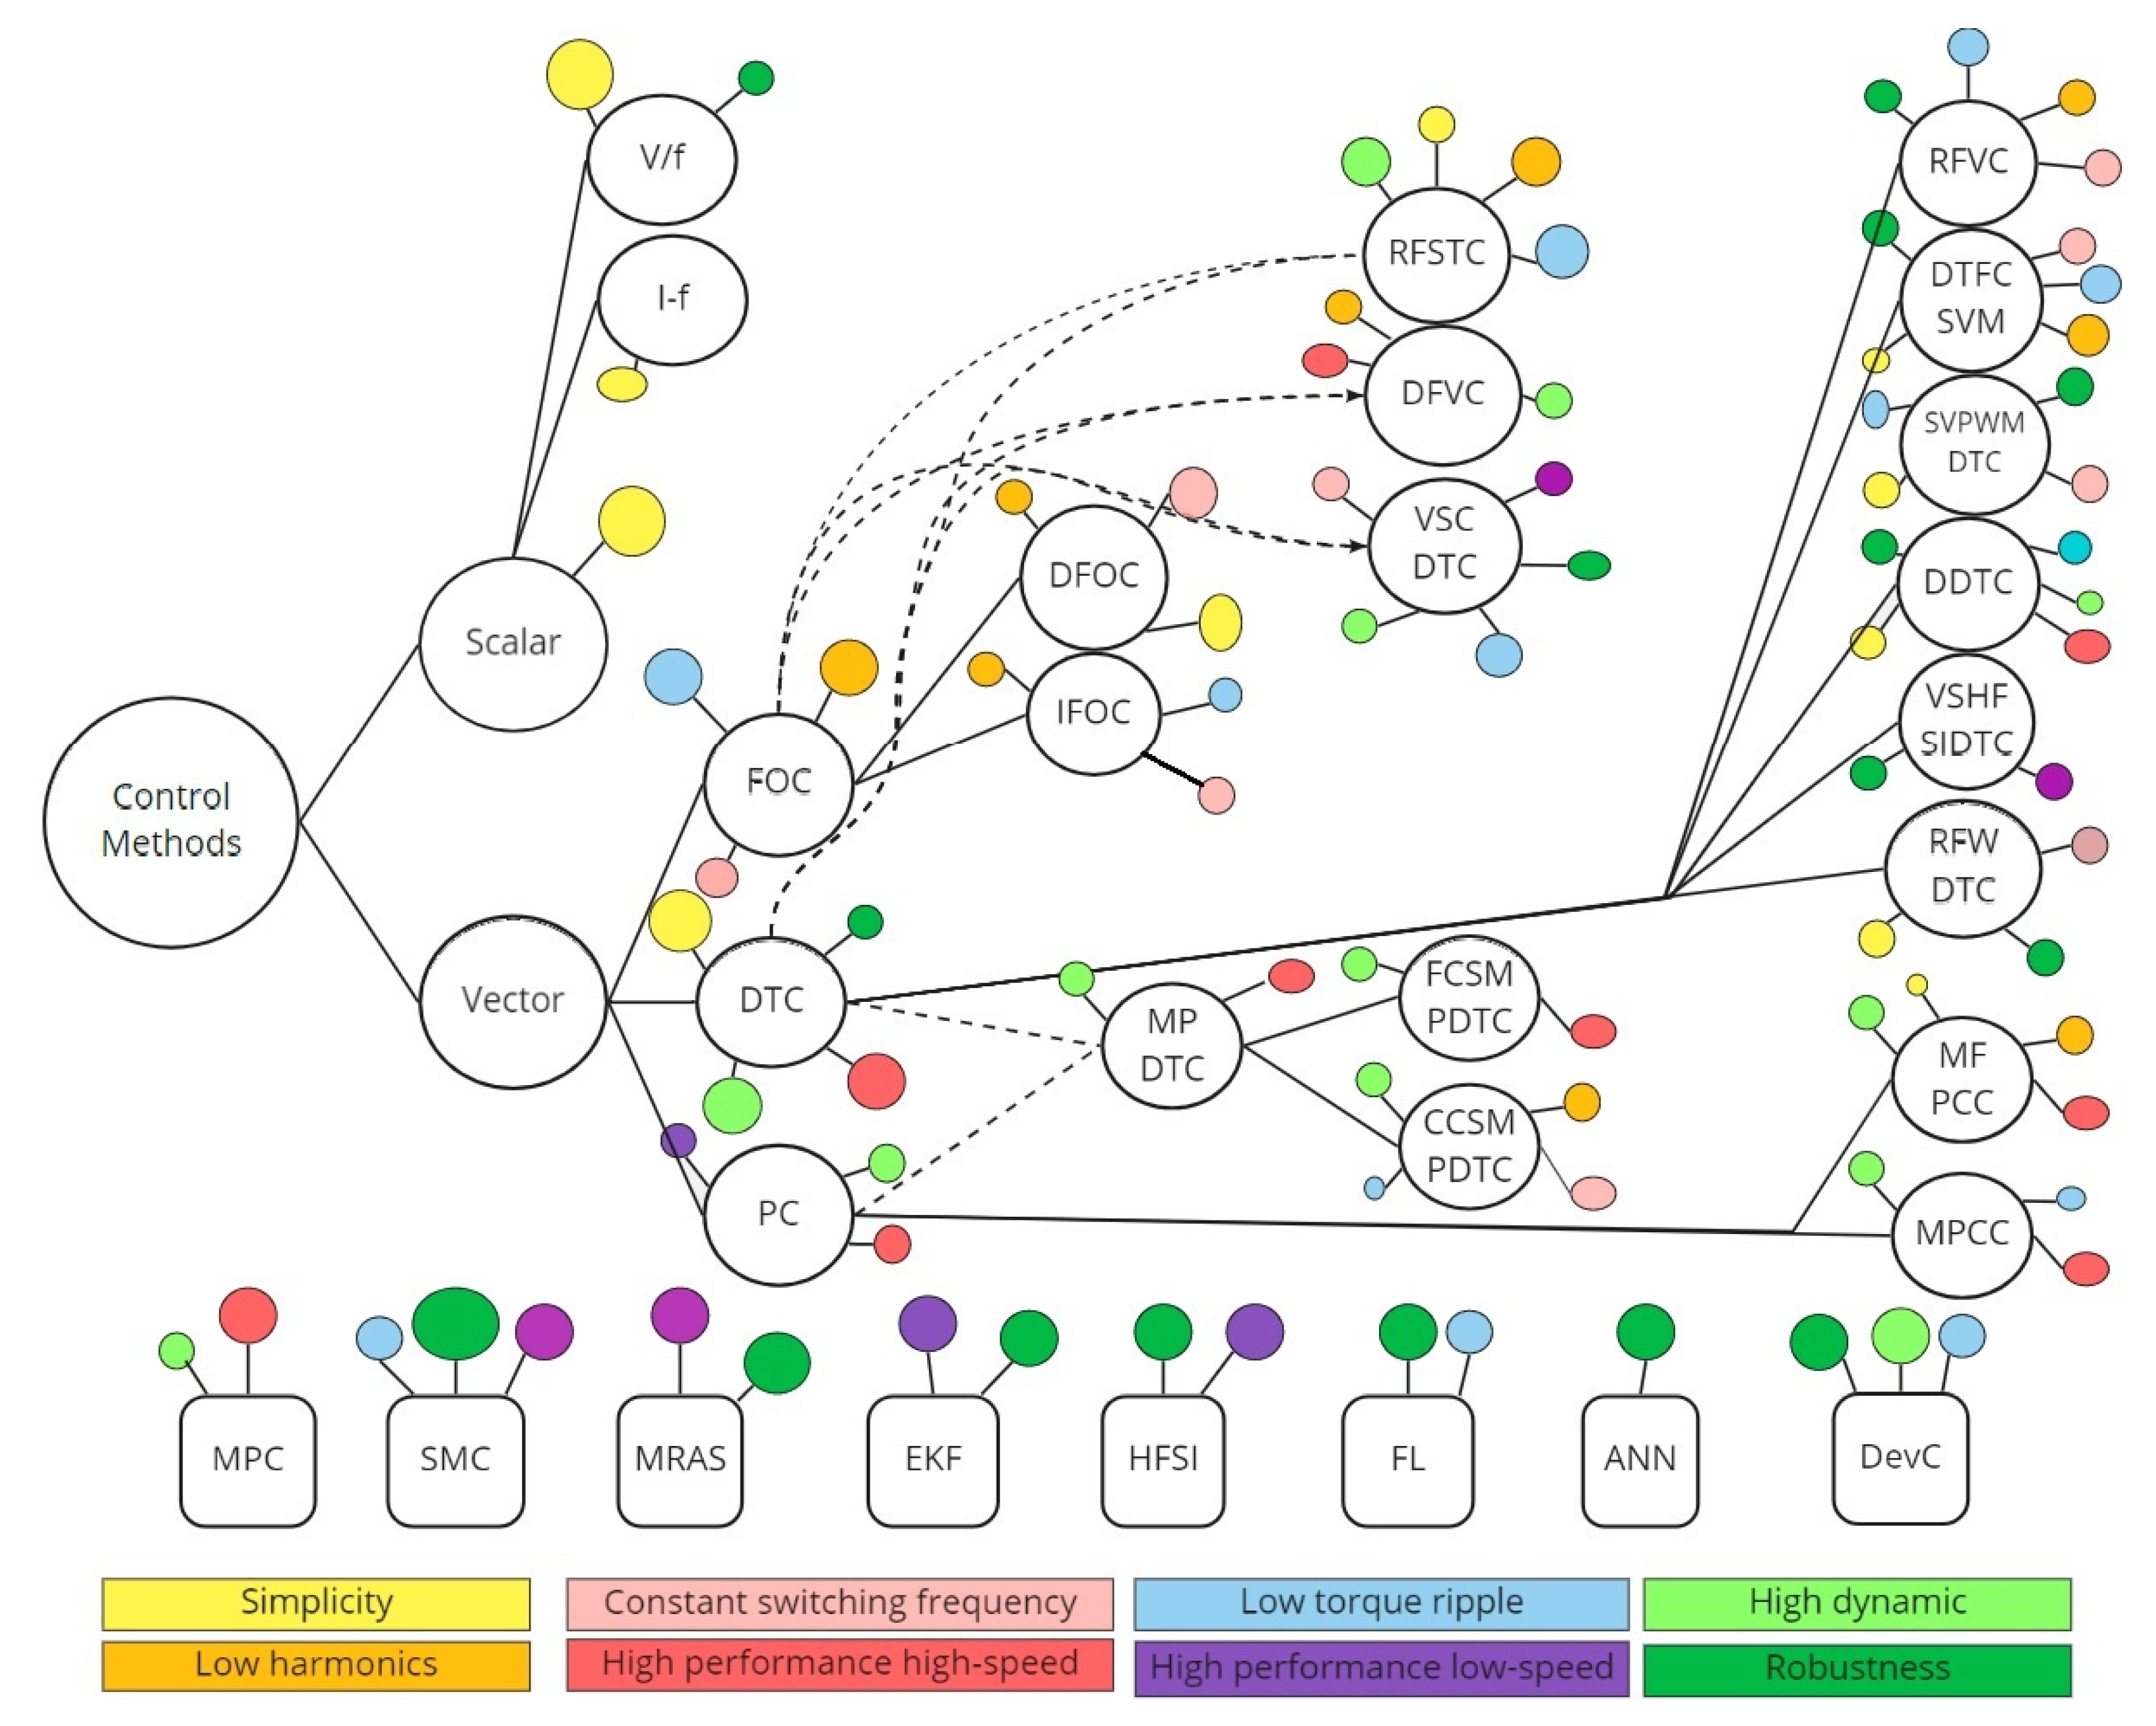
\includegraphics[width=0.70\textwidth]{src/png/control-strategies-diagram.png}
            \caption{Control strategies used for Synchronous Reluctance Motors (\gls{abbreviation:synrelm}). \cite{heidari-a-review-of-synchronour-relucatence-motor-drive-advancements}}
            \label{fig:control-strategies-diagram}
        \end{figure}

\section{Comparison to other machines}
    When designing electric drives there are numerous options on which motor to use in the designed application. A~comprehensive comparation study was well carried out in \cite{zhang-Comprehensive-Comparative-Study-on-Permanent-Magnet-Assisted-Synchronous-Reluctance-Motors-and-Other-Types-of-Motor}. Authors compare the induction machine (\gls{abbreviation:im}), synchronous reluctance motor (\gls{abbreviation:synrelm}), permanent magnet assisted synchronous reluctance motor (\gls{abbreviation:pmsynrelm}) and interior permanent-magnet machine (\gls{abbreviation:ipm}).\par
    The machines are compared based on the design parameters regarding their electromagnetic performance, material cost and temperature. The authors in \cite{zhang-Comprehensive-Comparative-Study-on-Permanent-Magnet-Assisted-Synchronous-Reluctance-Motors-and-Other-Types-of-Motor} conclude, that the electromagnetic performance of analyzed ferrite-based \gls{abbreviation:pmsynrelm} is better than that of the \gls{abbreviation:im} and \gls{abbreviation:synrelm} which does not use in their design any \gls{abbreviation:pm}s. The cost of used materials for \gls{abbreviation:pmsynrelm} is lower than for the \gls{abbreviation:ipm}. But the torque ripple and the demagnetization of ferrites may be a problem when using the \gls{abbreviation:pmsynrelm}. \cite{zhang-Comprehensive-Comparative-Study-on-Permanent-Magnet-Assisted-Synchronous-Reluctance-Motors-and-Other-Types-of-Motor}

\newpage
\section{Recent research interest}
    In recent years the research of \gls{abbreviation:pmsynrelm} has been focused on improving the overall performance, cost and behaviour of permanent magnet assisted machines.\par
    The improvement was achieved:
        \begin{itemize}
        \item by using non-rare earth materials such as ferrites,
        \item by using novel hybrid stator winding structures,
        \item by analyzing rotor structure types and motor parameters based on the permanent magnet position and perfecting the design for the specific application.
        \end{itemize}

    Some research articles focus on improving well known control strategies to achieve better performance of the drive. When using ferrite based permanent magnets the main concern of the applied control strategies is to minimize (better eliminate) the possibility of a permanent demagnetization which could occur.\par
    New types of motors and control strategies are proposed in \cite{ostovic-Memory-motors-a-new-class-of-controllable-flux-PM-machines-for-a-true-wide-speed-operation}. Proposed motors utilize variable flux strategy where high magnitude of stator current $i_d$ for a short amount of time may cause that the ferrite based permanent magnets are demagnetized. When the demagnetization is not needed the stator current $i_d$ may cause the re-magnetization of permanent magnets. The proposed principle is still being developed and published about.


\flushbottom % vyčištění stránky

% konec závěru

\newpage
\setmonofont{Times New Roman}

%% REFERENCES %%
\printbibliography[title={{References}}]	
\nocite{*}
\setmonofont{CourierPrime-Regular}
\addcontentsline{toc}{section}{\numberline{}References} % Adding citations to TOC %

%% APPENDIX %%
\appendix
\titleformat{\section}{\color{ctublue}\fontspec{Times New Roman}\fontsize{15}{15}\bfseries}{Appendix \thesection:}{2.1em}{}

\begin{appendices}
	\section{List of symbols and abbreviations}
    \vspace*{0.25cm}
		\printglossary[type=abbreviationslist, style = myStyleAbbreviations]

		\FloatBarrier
		%\newpage
		\printglossary[type=symbolslist, style =  myStyleSymbols]

	\end{appendices}
\end{document}
